
\documentclass{MScthesisITEM}

% this package is just to generate text for demo-purposes
\usepackage{blindtext}
\usepackage{subcaption}
\usepackage{rotating}
\usepackage{pgfplots}
\usepackage{listings} 
\usepackage{pdfpages}
\newtheorem{cnj}{Conjecture}

\title{Cyber Insurance \& Insurable Topologies} % The title of your assignement; NB use \newlinetitle to start a newline
\author{Håvard Råmundal Halse \\ Jonas Hoemsnes} % Your firstname and lastname
\supervisor{Gergely Biczók, Postdoc}
\professor{Jan A. Audestad, Professor II} % Affiliation = ITEM for instance

%% Uncomment the following in case you want subfigures; note that there will be a warning for the caption package
% \let\subcaption\undefined
% \let\subfloat\undefined
% \usepackage[bf]{caption}
% \usepackage{subcaption} 
\DeclareGraphicsExtensions{.pdf,.jpg}
\graphicspath{{./figs/}}
\loadglsentries{glossary}
\makeglossaries
\setcounter{secnumdepth}{2}
\setcounter{tocdepth}{4}

\begin{document}
\selectlanguage{english}
\titleITEM
\pagenumbering{roman}
\pagestyle{plain}
%% Only for the project
%\titleITEM gfgfg

%% Only for the master's thesis; for the project report the description is taken from It's Learning and added by the department
% \selectlanguage{english} % Change to 'norsk' if you are writing in Norwegian
 \begin{titlingpage}

\noindent
\begin{tabular}{@{}p{4cm}l}
\textbf{Title:} 	& \thetitle \\
\textbf{Students:}	& Håvard Råmundal Halse \& Jonas Hoemsnes \\
\end{tabular}

\vspace{4ex}
\noindent\textbf{Problem description:}

Security breaches are increasingly prevalent in the Internet age causing huge financial losses for companies and their users. Cyber-insurance is a powerful economic concept that could potentially help companies in the fight against such malicious behavior. Earlier research suggests that cyber-
insurance has failed to reach its promising potential, although the concept has been around since the 1980s. Researchers have proposed and analyzed several functional models of cyber-insurance in order to cope with or mitigate its unique characteristics: Interdependent security, correlated risk and asymmetrical information. However, the cyber-insurance market is still in a dormant phase.

A specific problem with cyber-insurance is determining the overall risk of the network structure to be insured. If cyber-insurance networks were describable and analyzable through graphs, the calculation of overall risk would be much easier. Are there specific graphs with properties that will help improve the market? Is it possible for insurers to incentivize companies forming networks with such beneficial graph structure or transforming existing networks into these superior structures?

The students will:

\begin{itemize}
 
\item conduct a background study and a market survey to validate the current state of cyber-insurance
\item study and characterize graphs with desirable properties regarding cyber-insurance
\item build and analyze a model of network formation which gives rise to such network structures
\end{itemize}


\vspace{2ex}

\noindent
\begin{tabular}{@{}p{4cm}l}
\textbf{Supervisor:}			& \thesupervisor \\
\textbf{Responsible professor:} 	& \theprofessor \\
\end{tabular}

\end{titlingpage}
% \cleardoublepage

%% There must be an abstract in English, even though the main text is in Norwegian
\selectlanguage{english}
\pagestyle{empty}
\begin{abstract}
Cyber-insurance is a powerful economic concept that can help companies in a world where cybercrime exist. From the early 80s, several researchers claimed that cyber-insurance had a bright future, and could become an important economic tool for handling residual cyber-risks.

The market study for this thesis revealed that both the European and US cyber-insurance market have failed to become a relevant factor for the ICT industry. Even though the US market has matured more than the European market, they are both far away from realizing their potential. Innovative approaches to handle the unique problems of cyber-insurance are needed.

This thesis takes a new approach towards solving some of the problems of cyber-insurance. First, network structures with properties that made them superior as cyber-insurance networks were found and characterized. Then several models for forming these network structures were introduced and analyzed using game theory and a simulation tool called Netlogo. In every model, new properties that relate the model to the real world and real-world insurance products are introduced. The results show that insurers can use the insurance premium as a tool for determining the resulting formation of the network. If the insurance premium is set to the right level, these superior structures will evolve. 

We believe our findings could help the cyber-insurance market evolve, by giving insurers a proper tool to better analyze and control formation of cyber-insurance networks. 

Further work should try mapping our models and simulations to real-world networks more extensively. This could be achieved by finding and introducing more realistic risk functions, and by letting nodes choose their neighbors by preference, not randomly. 

\end{abstract}
\cleardoublepage

%% Only for the master's thesis; if the main text is in English and you can write Norwegian, there must be an abstract in Norwegian as well.A
% \selectlanguage{norsk}
% \pagestyle{empty}
\renewcommand{\abstractname}{Sammendrag}
\begin{abstract}
\noindent Cyberforsikring er et kraftfullt økonomisk konsept som kan støtte bedrifter i en verden full av nettkriminalitet. Forskere har fra starten av 80-tallet spådd en lys fremtid for cyberforsikring, og har ment at det kunne bli et viktig økonomisk verktøy for å håndtere cyberrisiko.

Markedsundersøkelsen i denne oppgaven avdekket at hverken det europeiske eller det amerikanske markedet for cyberforsikring har greid å bli en viktig faktor i IKT-industrien. Selv om det amerikanske markedet er noe bedre utviklet enn det europeiske, så har begge langt igjen. Det trengs nye og innovative framgangsmåter for å håndtere de unike problemene knyttet til cyberforsikring.

Denne oppgaven presenterer en ny tilnærming for å prøve å løse noen av problemene knyttet til cyberforsikring. Først ble nettverksstrukturer med egenskaper som gjorde dem spesielt godt egnet som cyberforsikringsnettverk funnet og definert. Deretter ble flere modeller for å skape disse nettverksstrukturene introdusert og analysert gjennom spillteori, og ved bruk av simuleringsverktøyet «Netlogo». I hver modell ble så nye egenskaper introdusert, der hver egenskap kunne relateres til den virkelige verden og til virkelige forsikringsprodukter, slik at modellene ble mer realistiske. Resultatene viste at forsikringsselskapene kan bruke forsikringspremien som et verktøy for å bestemme den resulterende nettverksformasjonen. Hvis forsikringspremien blir satt til riktig nivå, så vil de spesielt godt egnete nettverksstrukturene oppstå. 

Vi mener at våre modeller og resultater kan hjelpe cyberforsikringsmarkedet til å utvikle seg, og vil kunne gi forsikringsselskaper et egnet verktøy til å analysere og kontrollere hvordan cyberforsikringsnettverk oppstår.

Fremtidig arbeid bør søke å la modellene og simuleringene i denne oppgaven nærme seg den virkelige verdens nettverk ytterligere. Dette kan gjøres ved å finne og introdusere mer realistiske risikofunksjoner, og ved å la noder opprette linker etter preferanse heller enn tilfeldig.

\end{abstract}
% \cleardoublepage

\selectlanguage{english}% Change to 'norsk' if you are writing in Norwegian

\renewcommand{\abstractname}{Preface}
\begin{abstract}
This study serves as a master thesis in the 10\textsuperscript{th} semester of our Master of Science degree in Communication Technology at the Norwegian University of Science and Technology. 

We would like to thank everyone who has contributed and supported our work throughout this semester.
A special thanks is given to our supervisor Gergely Biczók, Postdoc at the Department of Telematics (ITEM), for valuable feedback,
ideas and guidance during the project period.
\\
\end{abstract}

\begin{center}
Håvard Råmundal Halse \& Jonas Hoemsnes \\Trondheim, Norway \\ June, 2013
\end{center}



\cleardoublepage

% similarly you may add a separate acknowledgments page

\tableofcontents*
\cleardoublepage

%% include if relevant
\listoffigures
\cleardoublepage

%% include if relevant
%\listoftables
%\cleardoublepage

%% include if relevant
%\listofalgorithms
%\addcontentsline{toc}{chapter}{List of Algorithms}
%\cleardoublepage

%% include if relevant
%\printglossary[title=List of Symbols, style=long]
%\cleardoublepage
%\glsaddall[]

%% include if relevant
%\printglossary[title=List of Acronyms,type=\acronymtype] % prints just the list of acronyms
%\cleardoublepage

\pagenumbering{arabic}
\pagestyle{ruled}
%Part 1: Background

\chapter{Introduction to Cyber Insurance}
\label{chp:introductionToCyberInsurance} 

Cyber-insurance is an insurance product used to transfer financial risk
associated with computer and network related incidents over to a third party.
 Coverages provided by cyber-insurance policies may include property loss and
  theft, data damage, cyber-extortion, loss of income due to denial of

   service attacks or computer failures. \cite{washingtonPaper}

  
    Cyber-insurance works the same way as traditional insurance, where the insurance contract (policy) binds the insurance company to pay a specified amount to the insurance holder when certain incidents occurs. In return, the insurance holder has to pay a fixed sum (premium) to the insurance company. \cite{enisarapport}

  Traditional coverage policies rarely cover these incidents, therefore 
   cyber-insurance is seen as a huge potential market. However, the concept 
   of cyber-insurance has been around since the 1980s, but so far it has failed to reach its promising potential. 
   
 
   
 



\\
\\
One problem with cyber insurance is actors see it as a solution to the problem of being secure. Instead of investing in security, they now have a way of buying 
their way out. However, this problem might solve it self due to the fact that insurance companies only will indemnify the losses where victim can prove that a certain event has occurred. When it comes to cyber insurance, one often need computer forensics to generate the evidence needed. 






%\Blindtext[3][1]

%\begin{figure}
%\centering
%% dummy figure replacement 
%\begin{tabular}{@{}c@{}}
%\rule{.5\textwidth}{.5\textwidth} \\
%\end{tabular}
%\caption{\label{fig:example}A figure}
%\end{figure}

%\section{First section}\label{sec:first_section}

%\subsection{First subsection with some \texorpdfstring{$\mathcal{M}ath$}{Math} symbol}\label{sec:first_ssection}

%\blindtext
%\begin{itemize}[topsep=-1em,parsep=0em,itemsep=0em] % see http://mirror.ctan.org/macros/latex/contrib/enumitem/enumitem.pdf for details about the parameters
% \item item1
% \item item2
% \item ...
%\end{itemize}

%\subsection{Mathematics}

%\blindmathtrue
%\blindtext

%\begin{proposition}\label{def:a_proposition}
%A proposition... (similar environments include: theorem, corrolary, conjecture, lemma)

%\end{proposition}

%\begin{proof}
%\vspace*{-1em} % Adjust the space when parskip is set to 1em
%And its proof.
%\end{proof}

%\begin{table}
%\caption{\label{tab:example}A table}
%\centering
%\begin{tabular}[b]{| c | c | c | c | c |}
%\hline
%a & b & c & d & e \\ \hline
%f & g & h & i & j \\ \hline
%k & l & m & n & o \\ \hline
%p & q & r & s & t \\ \hline
%u & v & w & x & y \\ \hline
%z & æ & ø & å &   \\ \hline
%\end{tabular} 
%\end{table}

%\subsection{Source code example}

% \floatname{algorithm}{Source code} % if you want to rename 'Algorithm' to 'Source code'
%\begin{algorithm}[h]
%  \caption{The Hello World! program in Java.}
%  \label{hello_world}
  % alternatively you may use algorithmic, or lstlisting from the listings package
%  \begin{verbatim}
  
%class HelloWorldApp {
%  public static void main(String[] args) {
%    //Display the string
%    System.out.println("Hello World!");
%  }
%}
%\end{verbatim}
%\end{algorithm}

%You can refer to figures using the predefined command like \fref{fig:example}, to pages like \pref{fig:example}, to tables like \tref{tab:example}, to chapters like %\Cref{chp:example} and to sections like \Sref{sec:first_section} and you may define similar commands to refer to proposition, algorithms etc.

\chapter{Current market}
\label{chp:hvahardenneaasi??} 
carriers in London, New York, Zurich, Bermuda, Europe, the U.S. and 
elsewhere developing cybersecurity insurance products for their clients
Lots of challenges for cybersecurity insurance, both buyers and sellers. 
Buyers face tremendous confusion about cyber risks and their potential impacts on business. 
people dont know or understand what kinds of risk cyber inlcudes, 
how large losses can be and why should they care about externalities?
over 50 carriers in the cybersecurity insurance market today that offer a wide variety of products.
\cite{Cyberworkshop}
\subsection{Cost of cyber crime}
Despite the widespread awareness of cyber crimes, cyber attacks occur frequently. The companies studied in \cite{ccost} experienced successfull every week. A successfull cyber attack can result in serious financial consequences. And the longer it takes to resolve the attack, the more costly it get. This paper found that the median cost of cyber crime is \$5.9 million per year, ranging from \$1.5 million to \$36.5 millon per company, which is an 56 percent increase from the last year. With these numbers in mind, cyber insurance should be a very attracting security investment. There are more and more insurance companies offering cyber protection, but there are still many companies not utilizing them. \cite{compworld}

Cyber crime is growing, the costs of cyber crime are also increasing.
\include{relatedwork}
\chapter{Graphs and Network Formation}
\label{chp:graphTheory} 

In nature and our society there are lots of scenarios that can be described using graphs. A range from infrastructure, such as railroads, water pipelines and electricity grid, to societal relationships, disease epidemics can all be visualized using graphs. Cyber-insurance is no exception, and can also be structured as a graph. This is of interest because, when one can describe a phenomenon with graphs, it is much easier to analyze and find its characteristics. Hence the graph therefore serves as an analytic tool \cite{audestad}. 

Several studies have been done on the characteristics of different graphs, such as E-R graphs and A-B graphs (scale-free graphs) which is thoroughly described in the methodology chapter. In addition, one have found special characteristics on star-shaped graphs and cliques. This chapter will highlight which characteristics are desirable to have in the cyber-insurance market, and point out the structures that possess these characteristics. The results found here will serve as the foundation of our modeling work, where we try to force these graph structures to emerge endogenously. 
 
\section{Real world graph structures}
As a starting point lets have a look at a couple of real world examples of how complex systems with huge amount of data could be structured as graphs. We will see how complex structures becomes rather intuitive when presented as a graph. By looking at the graph structure, one can determine what type of graph that appears, and hence certain characteristics will apply.  

\subparagraph{Stock markets.} The research paper \cite{greekStockMarket}, analyzes the correlation between different stocks in the Greek stock market in year 1997. They compared the daily closing price of stock $i$ at day $t$, and compared the similarity of a pair of stocks $i$ and $j$ by using the correlation coefficient. The idea is that the correlation coefficient between a pair of stocks can be expressed using different distances in a graph structure. A short distance means high correlation and long distance means low correlations between the stocks. Normally this network would be shown as a fully connected graph, which will consist of $\frac{n(n-1)}{2}$ edges, and would be difficult to analyze. However the approach taken in the paper will present a clear understandable graph consisting of $(n-1)$ edges showing the correlations between the stocks.

The resulting graph can be seen in Figure \ref{fig:greekStockMarket}, and show a network consisting of several clusters linked together. Instead of having to analyze a complex system with huge amount of data, the stock market can be analyzed by its topological properties, such as the high clustering coefficient, i.e a star-topology, which will among others point out which stocks have the most influence on others. 
\begin{figure}[h]
\centering
\begin{tabular}{@{}c@{}}
\includegraphics[width=1.0\textwidth]{../Figures/greekStockMarket.jpg}
\end{tabular}
\caption[Caption for LOF]{Network obtained by comparing two stocks correlation coefficient in the Greek stock market (Athens Stock Exchange, ASE) in year 1997. The different colors represent the different sectors of economic activity \cite{greekStockMarket}.
\label{fig:greekStockMarket}}
\end{figure}

\subparagraph{Airline routes.}
Another real world network which shows the same characteristics as scale-free graphs is the map of airline routes. Figure \ref{fig:airlineRouteMap} shows the US route map of the American airline company, SkyWest. The characteristic clustering emerges in the figure, where a majority of the flights departs from either Denver, Chicago or San Francisco. Not surprisingly, these airports are all in the top 7 busiest airports in the US \cite{busiestAirports}, and serves as hubs for many of SkyWest flights. In the airline industry some airports are called hubs, because that's what they are, - a connection point for major parts of the network of flights. The network of flights, as depicted in Figure \ref{fig:airlineRouteMap} follows the characteristics for A-B graphs. Hence, as we also can confirm from looking at the graph, the network are vulnerable against direct attacks. This means that if an low edge degree airport is shut down, there will be little consequence for the rest of the network. However, if one of the hubs is forced to close, it will provoke huge delays through out the whole network of flights, because many of the destinations are interconnected via the hubs. 


\begin{figure}[h]
\centering
\begin{tabular}{@{}c@{}}
\includegraphics[width=1.0\textwidth]{../Figures/airlineRoutesUSA.png}
\end{tabular}
\caption[Caption for LOF]{SkyWest Airline combined route map \cite{airlineRoutes}.
\label{fig:airlineRouteMap}}
\end{figure}

Both examples can be characterized as a scale-free network, and often natural networks are scale-free. Since we are able to ascertain this we know for example that one will experience large consequences if a hub in the network stop functioning. 
This shows the strength of being able to structure systems as graphs. When a certain structure appears one can assume that the network will behave according to a set of rules. This is why we wish determine whether there are any structures that possesses preferred characteristics to be associated with cyber-insurance. Because then the work is reduced to find a proper way to force the formation of the given network structure.


\chapter{Evolutionary dynamics on graphs}
\label{chp:nature} 
\cite{lieberman2005evolutionary}
Tanker fra paper:

If advantegous mutant(f.eks virus) incerted in circulation graph, it will have a fixation probability 
\begin{equation}  p_{1}=\frac{(1-1/r)}{(1-1/r^{N})} \label{eq:fixation} \end{equation}
Isotherm graphs are a subgraph of circulation. 

If $W$ is symmetric, or isotherm then the fixation probability is allways \ref{eq:fixation}
isotherm means doubly stochastic, all rows and cols sum to 1. 
If a graph is one rooted, it has a fixation prob of $1/N$ regardless of $r$. If a graph has more then one root, its fixation probability is zero. 
Is it possible to find graphs with fixation probability that exceeds \ref{eq:fixation}? Is it possible to suppress drift and amplify selection?
In a star-topology \ref{fig:star} the fixation probability is\begin{equation}p_{2}=\frac{(1-1/r^{2})}{(1-1/r^{2N})} \label{eq:fixation2} \end{equation}.
or more generally: \begin{equation}
p_{k}=\frac{(1-1/r^{k})}{(1-1/r^{kN})} \label{eq:fixationk}
\end{equation}
And the selective difference is as we see amplified from $r$ to $r^{2}$. i.e. a star act as an evolutionary amplifier,
 favouring advantageous mutants and inhibiting disadvantageous mutants, tilts towards selection and against drift.
 in certain graphs, star, funnel, metafunnel, if N is large enough, fixation proability for advantageous mutant converges to 1. Fixprob for disadvantaeus converges to 0.
This could maybe be used to show that if we have a star, funnel, metafunnel or something, and we secure the nodes it could force the virus to die out?
Scale-free networks have most of their connectivity clustered in a few vertices, i.e. they are potent selection amplifiers.
More generalized, $W$ does not need to be stochastic, $w_{ij}>=0$. 
If the sum of all edges leaving a vertex is equal for all vertexes, then the graph will never suppress selection.
If the sum of all edges entering a vertex is equal for all vertexes, the graph never suppress drift.
If both then the graph is called a circulation.
 

\begin{figure}
\centering
\begin{tabular}{@{}c@{}}
\includegraphics[width=0.5\textwidth]{NetworkTopology-Star.png}
\end{tabular}
\caption{\label{fig:star} A star-topology}
\end{figure}












\chapter{Methodology}

\section{Graphs}
As mentioned in the previous chapter, graphs are good analytical tools when studying complex systems. Since we will use graphs extensively throughout this thesis, it is important to establish an understanding of basic graph properties. Figure \ref{fig:generalGraph} depicts the basics of an unweighted graph, where the edges are not assigned any value. Weighted edges can be useful to e.g. reflect capacity constraints such as a link's maximum bandwidth, or the length of a road (edge), but will not be used in this thesis. Other common definitions used when describing graphs are listed below \cite{audestad}:
\begin{itemize}
\item Edge degree: Number of edges connected with a node.
\item Hub: Node with high edge degree.
\item Cycle: A chain originating and terminating at the same node.
\item Cluster: Subgraph of highly connected nodes.
\item Cluster coefficient: Probability for two nodes to be adjacent to a third node.
\item Clique: Subgraph where all nodes are adjacent (cluster coefficient = 1).
\item Small world graph: Graph with small diameter and large cluster coefficient (e.g. the Internet and A-B graphs, described in section \ref{ABgraph}).
\end{itemize}

\begin{figure}[h]
\centering
\begin{tabular}{@{}c@{}}
\includegraphics[width=0.4\textwidth]{../Figures/generalGraph.png}
\end{tabular}
\caption{\label{fig:generalGraph} General graph \cite{audestad}.}
\end{figure}

\section{Random Graphs}
Cyber-insurance covers many fields, from financial transactions and software development to computer networks. Many of these fields share a common characteristic, they can all be described as a graph, and often as a random graph. Therefore, the study of random graphs is of special concern. The research on random graphs is fairly new compared to other mathematical discoveries. The first extensive results where found by Erdös and Rényi in 1959, hence the resulting structures were called  E-R graphs. Later and probably with more accurate results were the work of Albert-Barabási in 1999 \cite{audestad}, leading to the characterization of A-B graphs. 
\subparagraph{Erdös-Rényi Graphs.}
E-R graphs are networks created between a fixed number of $n$-nodes, where each node connects to another of the $n-1$ nodes with 
probability $p$. The resulting graph will on average contain $\frac{n(n-1)p}{2} \approx \frac{n^{2}p}{2}$ edges \cite{barabasi}. 
By analysing the graph, the authors found some interesting properties:

\begin{itemize}
\item If $p<n^{-2}$  then there is no edges in the graph. 
\item If $p=c/n$ where c is a constant between $1 < c < log\: n$, the graph will provoke a single large component to grow within the graph.
\item If $p>(ln\: n)/n$ then the graph is completely connected. 
\item If $p = 1/n$ triangles start forming in the graph. 
\end{itemize}

A fully connected E-R graph will have a short diameter similar to the Internet, and thus could be a very good description of structures similar to the Internet. However, the edge degree follows a Poisson distribution, which means that the edge degrees are peaking around the average value \cite{audestad}. E-R graphs do not capture the immense clustering coefficient which is present in networks such as the Internet. In other words, E-R graphs are not small world graphs, and a different graph structure is needed to model computer networks.
An interesting fact about these graphs is their vulnerability. These graphs are very vulnerable against random attacks, such as nature disasters, but robust against directed attacks. Due to the fact that if you remove all edges from one node, little damage is done, since the network is not dependent on only a few nodes. Every node has approximately the same node degree, and it is the sum of all the nodes' connections that creates the network.

\subparagraph{\label{ABgraph}Albert-Barabási Graphs.}
The structure which is believed to be most accurate for modelling computer networks are A-B graphs. A-B graphs are different from E-R graphs since they are scale-free, meaning that the vertices do not have a constant value throughout the entire graph. Albert and Barabási found that the edge degree of each vertex follows a power law distribution; meaning that the probability that the edge degree is $g$ is proportional to $g^{-\gamma}$
where $\gamma$ is usually a number between 2 and 3. This distribution is called a thick-tail distribution, because there is a significant probability that a node may have a very high degree \cite{audestad}.
These graphs are in contrast to E-R-graphs, very vulnerable to directed attacks, because if you take out a hub, mayor parts of the network will be affected. But the graph is very robust against random attacks, which is why most of the networks we observe in nature can be depicted as A-B-graphs.
A-B graphs can grow and become scale-free if every new node is connected to one or more already existing node with a probability proportional to the edge degree of that node. The paper present an algorithm that creates A-B graphs and Figure \ref{fig:ABgraphcreation} shows a graph that evolves from this algorithm:

\begin{itemize}
\item A new single vertex is added to the graph.
\item This vertex is connected to exactly two other vertices in the graph.
\item The probability that the new vertex connects to another vertex is dependent on the edge degree of the other vertex, higher edge degree meaning higher probability
\item There is only one edge between two vertices.
\end{itemize}


\begin{figure}[h]
\centering
\begin{tabular}{@{}c@{}}
\includegraphics[width=0.8\textwidth]{../Figures/ABgraphcreation.png}
\end{tabular}
\caption{\label{fig:ABgraphcreation} Forming an A-B graph in 15 generations \cite{audestad}.}
\end{figure}

In addition to the high clustering coefficient Albert-Barabási showed that A-B-graphs have a fairly small diameter,
 which can be seen in Figure \ref{fig:ABgraphcreation}. 
The World Wide Web, neural networks, scientific referencing, co-authorship and many other types of networks are very similar to A-B graphs \cite{audestad}.

\section{Game Theory}
Here we will present some of the game theory concepts used in our models, for more thorough explanation of game theory, see: \cite{nisan2007algorithmic, watson2008strategy}.
\subparagraph{One shot game.}
This type of game assumes that players act at the same time instantly, therefore there is no causality. A game in strategic (normal) form can be described by three elements:
\begin{itemize}
\item the set of players $i \in I$, which we take to be the finite set ${1,2,....,I}$.
\item the pure-strategy space $s_{i}\in S_{i}$ for each player i, where $s_{i}$ is a possible action of player i.
\item and payoff functions $U$, which give the players utility functions for each profile $s=(s_{1},s_{2},...,s_{I})$ of strategies.
\end{itemize}
A general solution concept for games of economic interest is the Nash Equilibrium solution. A Nash Equilibrium is a profile of strategies such that each players strategy is a best response to the other player's strategies. 
\subparagraph{Nash Equilibrium.}
A pure strategy profile $s^{*}$ is a Nash equilibrium if, for all players $i$
\begin{equation}
U_{i}(s^{*}_{i},s_{-i}^{*})\geq U_{i}(s_{i},s^{*}_{-i}) \in S_{i}
\end{equation}

\subparagraph{Subgame-perfect equilibrium.}
A strategy profile $s$ is a subgame perfect equilibrium if it represents a Nash Equilibrium of every subgame of the original game.
\subparagraph{Socially optimal.}
A socially optimal outcome is the set of choices that maximizes the sum of all players' payoffs. 
\subparagraph{Price of Anarchy.}
The price of Anarchy (PoA) of a network game, measures the efficiency of the network, by comparing the equilibrium outcome with the socially optimal outcome. The reason for this possible inefficiency is that agents act selfishly and do not necessarily consider other agents' payoff when choosing an action. In our thesis, the price of anarchy will be a number between 0 and 1, where 1 is the socially optimal outcome.
\subparagraph{Stackelberg.}
Also known as a leader-follower game, it introduces multiple stages. The leader commits himself first, chooses his strategy, then the followers respond sequentially. The Stackelberg model can be solved to find the subgame perfect Nash Equilibrium, i.e. the strategy profile that serves each player best, given the strategies of the other players and that entails every player playing in a Nash Equilibrium in every subgame.
\subparagraph{Bayesian game.}
In Bayesian games, information about the other players' characteristics is incomplete. In these types of games, there is one player(the agent) who knows both types, and another player (the principal) who does not know the type of the other player. There are two types of equilibriums in this game:
A pooling equilibrium, is an equilibrium where both types of the agent choose the same action, i.e. the principal is not able to distinguish the two types. 
A separating equilibrium is an equilibrium where the agents of different types choose different actions, and thus the principal is able to determine the agent's type by observing his actions.
\subparagraph{Pairwise stability.}
A graph is pairwise stable if:
 \begin{enumerate}
\item \textit{No node wishes to delete a link he is involved in.}
\item \textit{If there exists a node which wants to add a link, then the node at the other end of the link does not want to establish this link.}
\end{enumerate} 
Pairwise stable networks are robust to one-link deviations, where link
severance is unilateral, while link creation is bilateral and under mutual consent of the two involved
players \cite{calvo2009pairwise}.

\section{Netlogo}
In addition to analyzing the different models with game theory, we created a simulator for the models, in a program called Netlogo. Netlogo is a programmable modeling environment for simulating natural and social phenomena. It is well suited for modeling complex systems developing over time \cite{netlogo}.
Netlogo is well suited to model our complex network formation games, and at the same time Netlogo provided us with a good graphical user interface that enabled us to see the result of the games, and also to easily adjust the different parameters. It was especially of use when facing models that were difficult to analyze, because it gave us a good graphical result, showing how the network evolved, and the final resulting network.  
In Figure \ref{fig:netlogo} we see the user interface, which is used to set up the parameters, start the modeling, and showing the resulting network formation. Figure \ref{fig:netlogo-code} shows how the coding interface looked like. For detailed overview of the code used in our different models, see appendix.
\begin{figure}[h]
\centering
  \includegraphics[width=0.9\linewidth]{../Figures/netlogoexample.png}
  \caption{\label{fig:netlogo} The figure shows a screen capture of Netlogo, while we are running one of our simulations.}

\end{figure}
\begin{figure}[h]
\centering
  \includegraphics[width=0.9\linewidth]{../Figures/netlogocodeexample.png}
  \caption{\label{fig:netlogo-code} The figure shows how the code interface in netlogo looks like.}

\end{figure}





%Part 2: Contributions/Modelene vaare

\chapter{Modeling Cyber-Insurance }
\label{chp:modelingCyberInsurance} 

In many scenarios nodes seeks to create networks in order to directly benefit from each other. The established links might represent companies out sourcing part of their manufacturing, or cooperative agreements in the development of new software products. In addition to increase the trade-off, each of the established links represents risk of being a victim of cascading failures. The intuitive example is the spread of epidemic diseases, also node failures of a power grid and financial contagion such as the one back in 2008 was a result of cascading failures. Strategic network formation using cyber-insurance can be used to prevent such situation in addition to increase the overall payoff of participants in a clustered network.

When deciding whether to establish connection to a neighbor agent, the payoff has to be higher in the balance between the expected earnings and the risk of the other party failing to complete the transaction. This is the reason why we seek to only download content from trusted peers and outlaw MC-gangs are consistently skeptical to enter into new agreements despite promising increased earnings, since the risk of undercover police are too high. 

The model from \cite{contagion} described in the related work chapter introduces a model where each node benefit from direct links to other nodes. However establishing a link will expose them to a risk if the node is not protected. Information about other nodes status (in our case, insured or not) will help nodes to guarantee cliques consisting of only the insnured nodes. According to the paper, such cliques will result in super critical payoff for every node connected. 
\subparagraph{Insurable topology}
One of the problems with cyber-insurance is to define and calculate the risks, because the network structure is undefined. If an insurer where able to predict the network structure, the calculations of overall risk would be realizable, and even better if the insurer where able to force some more robust network structures to evolve. 
Examples of such structures are as described in the graph theory chapter, scale-free network, which have been proven to be very robust against random attacks. Star-topologies, or star-like topologies such, which have a fixation probability that exceeds the fixation probability of circulation graphs. Star structures also have the nice property of minimizing the average path length, i.e. minimizing the cost spent on establishing links.
In our thesis we define an insurable topology as a structure which enables the insurer to calculate the overall risk, i.e. a structure who can be analyzed by the insurer.
The two main types of insurable topologies we will focus on are the clique and star-like structures. Since both of these have been identified to have calculable fixation probability. They also have other properties that are desirable for the insurer, such as the possibility of amplifying or suppress selection and drift. This is very desirable, because if the insurer is able to ensure that the nodes have a certain security level, especially the center node, then he can ensure that viruses does not spread.
The clique has the nice property of being able to achieve super critical payoff, as showed in \cite{contagion}. 


\subparagraph{Introduction to the modeling.}
There are many examples of nodes needing to establish connections, one example is a company needing to out-source certain tasks to remain competitive. This outsourcing involves some risks, such as, will the company deliver at the reported time, to the reported costs, what happens if they fail to deliver, what if they go bankrupt etc. If the companies that are going to establish links(cooperative contracts), know that the other firms are insured, it will be more secure and reliable to enter into an cooperative agreement. In this way trusted cliques can evolve. The firms benefit from connecting to other insured firms, and the insurance company can offer fair prices to the insured companies, because the risk is calculable in a trusted clique.

So our goal with the models are to find out how and when different networks evolve, and how the insurer can ensure that this will happen, by adjusting the parameter he can control, the insurance cost. 

Inspired by this model, we are step wise building our own model which shields light on how cyber-insurance can be used in network formation games to prevent cascading failures and increase an agents payoff.  
Through out this chapter new features will be added to the models, starting at the simple model-1, to make it more realistic and applicable, an overview of the different models can be seen in Figure \ref{fig:Overview-of-models}.

\begin{figure}[h]
\centering
  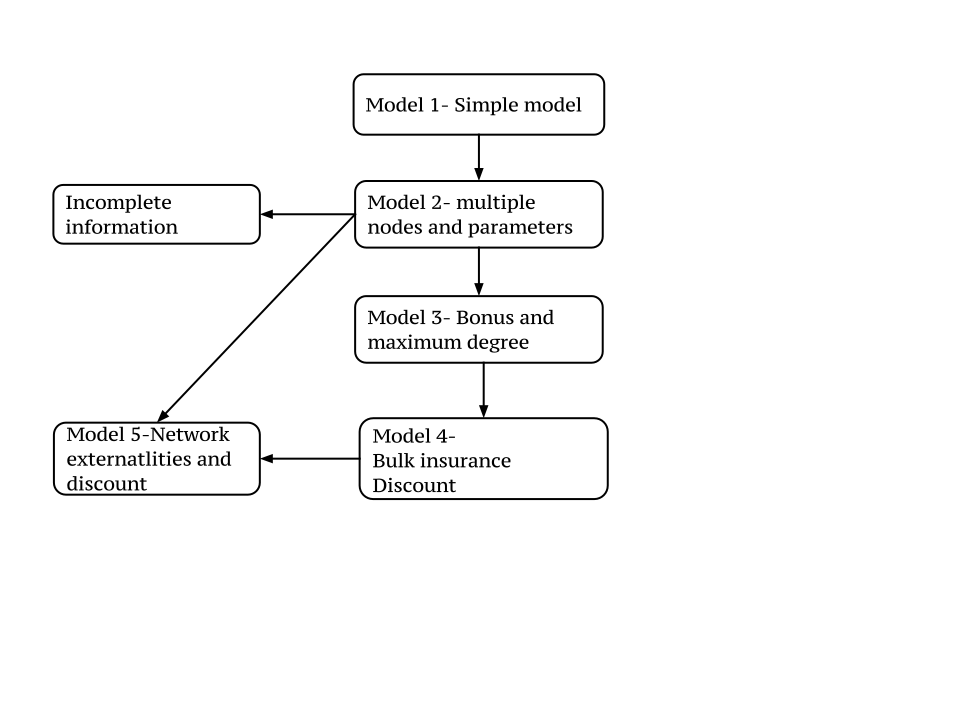
\includegraphics[width=0.9\linewidth]{../Figures/modeloverview.png}
  \caption{\label{fig:Overview-of-models} The figure show an overview of the different models we have created, and how they relate to each other. For every step, there are added some new features to the model.}

\end{figure}

\section{Model 1 - Initial Model \label{section:verysimplemodel}}

As a starting point the model is highly simplified in order to show the concept of how cyber-insurance can be used to create an insurable topology. We assume that every node has complete network information, i.e. it knows how many nodes that exists, and whether they are insured or not. The link establishment process is bidirectional, meaning both nodes must agree to establish the connection.

For the first model, we assume a set of $n$ nodes that are randomly chosen to be insured or not, as depicted in Figure \ref{fig:firstmod1}. They all get their own fixed income, and by connecting to other nodes they can increase their payoff. Non-insured nodes will have a risk of failure i.e. an expected cost of failure. Therefore if an insured agents chooses to connect to a non-insured nodes they will also suffer from this expected cost of failure. To simplify the decision process, the model follows a rule that only allows insured to connect to other insured agents and non-insured agents can only connect with each other. The resulting graph will be two fully connected cliques, one consisting of insured agents and the other of non-insured agents, as shown in Figure  \ref{fig:firstmod2}. 

This dichotomy represents a trusted environment for the insured nodes, because they know that each node in the clique is insured against risk. These nodes will benefit from each connection without having to worry about contagious risks from the connected nodes. 
A node in the non-insured clique will also experience a change in payoff from the links it has established, however each of the links has a probability of failure. Hence this environment is not trusted, and a link establishment will always involve some risk. 

The first model, although very simple, shows an insurable topology where insured agents benefit from being insured, and are candidates to receive super critical payoffs as described in \cite{contagion}.

\begin{figure}[h]
\centering
\begin{subfigure}{.5\textwidth}
  \centering
  \includegraphics[width=0.4\linewidth]{../Figures/firstModelWithNoParameters1.png}
  \caption{\label{fig:firstmod1} 15 Agents randomly choosen to be either insured (green) or non-insured (red).}
\end{subfigure}
\quad
\begin{subfigure}{.46\textwidth}
  \centering
  \includegraphics[width=0.8\linewidth]{../Figures/firstModelWithNoParameters2.png}
  \caption{\label{fig:firstmod2} Two clustered networks. One consisting of insured agents the other consists of non-insured.}
\end{subfigure}
\caption{\label{fig:firstmodfinal} Shows how agents connects to eachother according to model described in section \ref{section:verysimplemodel}.}
\end{figure}
 
\textbf{fjern dette?}
This model is very simplified and suffer from many limitations, among others it is too simple to reflect the dynamics of a real world scenario, where each node will have different variables with different values. Although it tries to deal with the problem of correlated risks and preventing free riders from entering the trusted clique (interdependent security problem), each node have a complete network information i.e. the problem with information asymmetry is not taken into account. 
\textbf{slutt paa fjern dette}

\section{Model 2 - Including Parameters}
The first model is highly simplified and suffer from many limitations, among others it is too simple to reflect the dynamics of a real world scenario, where each node will have different variables with different values. To improve this model we have to introduce parameters, that can be adjusted and reflects real world scenarios.
It is fair to assume that the insured nodes must pay an insurance premium, and this premium should be dependent on the number of links the node establishes. When two insured nodes establish a link between each other, they both have to pay a premium, this is to make the game more fair, and more realistic. For example if the two nodes had different insurance companies, then both companies would charge them for insuring the link.
When a node, insured or not, establish a link to a non-insured node, this involves a risk, and this risk will be represented as a expected risk cost. However if the changes in payoff when establishing a link is only negative, then no node would want to establish links. Thus the nodes will also receive a positive change in payoff when establishing different links. 

\subsubsection{Characteristics of the model}
The type of the nodes are given in advance, i.e. they are chosen to be insured or non-insured. The process of establishing link is a bidirectional decision. 
The insured nodes have to pay an insurance cost $I_{0}$, which represents the cost of signing a contract with an insurance company. I.e this could be an actual fee or a cost reflecting the work a player has to do to get a contract. The insurance premium is $I_{l}$, the expected risk cost is represented by $r$. $\beta$ represents the benefit of establishing a link.  
Table \ref{tbl:simplegamepara} presents an overview of the parameters. 
\begin{table}[h]
\centering
\begin{tabular}{lc}
 \hline
  $\beta$ - income from establishing a direct link \\
  $I_{o}$ - cost of having insurance. \\
  $I_{l}$ - increased insurance cost per link the node establishes\\
  $r$ - expected risk cost\\
  \hline
\end{tabular}
\label{tbl:simplegamepara}
\end{table}
\subsection{Two nodes scenario}
As a starting point lets look at the scenario involving only two nodes. In this game the strategy space of both players consist of four different strategies. A node can be insured or not, and choose whether to establish a link to the other node. I.e. the different strategies are: Be insured and establish link noted as: $IL$, 
be insured and not establish link: $I\overline{L}$. Not insured and establish link: $\overline{I}L$, and not insured and not establish link: $\overline{IL}$. It should be noted that since the decision to establish a connection is bidirectional, both have to choose a strategy where they want to establish a link, for the link establishment to be successful. Hence we end up with the game as shown in Figure \ref{fig:FirstGameTheoryModel}.

\begin{sidewaysfigure} 
\centering
\includegraphics[width=1.0\textwidth]{../Figures/FirstGameWithParameters.png}
\caption{\label{fig:FirstGameTheoryModel} Normal form game, showing the different strategies and the payoffs  for the different outcomes. The payoff are written in this order, A then B's. An agent has a strategy space of size 4. Maa ENDRES, FIKS NAVN IKKE FIRM, MEN NODE}
\end{sidewaysfigure}

As long as both $I_{l} \text{ and } r$ is less than $\beta$, the only nash equilibrium in Figure \ref{fig:FirstGameTheoryModel} is when both nodes chooses $\overline{I}L$. If we first look at node A, we see that when node B chooses $IL$, the best response is $\overline{I}L$, because $ \beta >\beta- I_{l}$ . And since the game is symmetric, the same holds for node B. 
When one of the nodes chooses $\overline{I}L$, the best response will be $\overline{I}L$, because $\beta - r>\beta - I_{l} - r  $. 
And thus the only nash equilibrium is when both nodes play $\overline{I}L$.

This means that two nodes will end up in a classic prisoner's dilemma\footnote{Prisoner's dilemma was originally framed by Merrill Flood and Melvin Dresher in 1950. The dilemma expresses a situation where two players each have two options whose output depends on the simultaneous choice made by the other. The original dilemma concerns two prisoners which separately decides whether to confess to a crime \cite{oxfordPrisonersDilemma}. It is a paradox in decision analysis which shows why two individuals might not cooperate, even if it is in their best interest to do so.}, where the best response is actually worse than the social optimal. In this case it is trivial to see that the social optimal scenario is for both nodes to choose $IL$, as long as $I_{l}<r$. However, the nodes will choose not to buy insurance. Or else they could risk ending up in a case where they pay $I_{l}$ without receiving any other benefit. 

  
\subsubsection{Solving the prisonersdilemma}
One possibility for solving the problem that the two nodes end up choosing not to acquire insurance is to introduce a leader follower game. In this game the players does not act at the same time, but in order, and they can observe the other players action.
If we consider a game with only two players, player one are the first to select an action. He chooses to insure or not. Then after observing this action player two chooses if he would like to insure or not. Then they choose if they would establish link or not, in the same order.
In this type of game the leader, will benefit from a first mover advantage, because he can now force the game in a direction he prefers, as long as:
\begin{equation}
I_{l}<\beta \text{ and } I_{l}>\beta-r \text{ and } r<\beta
\label{eq:stackelbergcondition}
\end{equation}
By finding all subgame equilibria in Figure \ref{fig:stackelberg} except the last one, i.e. the subgame where player one chooses to Insure or not, we get this subgame equilibria: $(L,\overline{L^{I}_{1}},\overline{L^{II}_{1}},L^{III}_{1}), (I_{2},\overline{I^{I}_{2}},L_{2}L^{I}_{2},\overline{L^{II}_{2}},L^{III}_{2})$
We have now analyzed the two different outcomes of player 1 choosing insure or not, thus he can now see what find his best response. The two options he can choose between are: Insure and get payoff $\beta-I_{l}$ or not insure and get payoff $\beta-r$. I.e. if $I_{l}<r$ player one will chose to insure, and thus forcing the game to end up in a equilibrium where both players insure and establish link. If the cost of insuring is higher than the expected risk cost $r$, then obviously there is no reason to choose insurance.
From this we see that if the insurance price are set to the right amount, the first player can force the outcome of the game to be the socially optimal outcome. 
The problem with this way of solving the problem is that it is very hard to solve for  multiple nodes, because the extensive form game becomes extremely complicated.

\begin{figure}[h]
\centering
  \includegraphics[width=0.9\linewidth]{../Figures/stackelberggame.png}
  \caption{\label{fig:stackelberg} Leader follower game, first player 1 chooses to insure or not, then player 2, and then they choose to establish link or not in the same order.}
\end{figure}


\subsection{Multiple nodes}
\subsubsection{Assumptions}
To improve the second model we now introduce a scenario with multiple nodes. As before the type is give, i.e each node is chosen to be either insured or not. The objective of this model is to find characteristic network formations that will evolve endogenously when the parameters are within certain conditions. Examples of characteristic networks of interest are cliques, scale-free and star networks.
We assume that every node has complete information of the network, i.e. every node knows the type of the other players. This is a very strong assumption, however in financial transactions and in cooperative software development networks, it is reasonable to assume that the parties can acquire this type of information prior to establishing a financial contract with each other.
\subsubsection{Analyzis}
As mentioned our goal is to find how and when certain network formations evolve. We know that if a node can increase his payoff by establishing a link, he will do so. Thus we can start analyzing the four possible link establishment scenarios, insured to insured, insured to non-insured, non-insured to insured, and non-insured to non-insured. 
Let $U_{i}$ denote the payoff of a node with degree $i$, and let $U_{i+1}$ be the payoff a node will receive if it establishes a new link.
\subparagraph{Insured to insured}
When two insured nodes are considering establishing a link, they will do so, if and only if both receive a higher payoff.  In this scenario the the payoff function of adding a link is as shown in Eq.(\ref{eq:itoimodel2}).
\begin{equation}
    U_{i+1}= 
\begin{cases}
    \beta - I_{l},& \text{if } i = 0\\
    U_{i}+\beta -I_{l},& \text{if }  i>0
   
\end{cases}
\label{eq:itoimodel2}
\end{equation}
In this scenario the condition shown in Eq.(\ref{eq:itoi-condition}) has to hold.
\begin{equation}
I_{l}<\beta
\label{eq:itoi-condition}
\end{equation}
\subparagraph{Non-insured to insured}
The payoff a non-insured receives by connecting to a insured is as described in Eq. (\ref{eq:noti-to-i-model2}). As we see this will allways be a positive change in payoff, and thus an non-insured node will always choose to connect to an insured node.
\begin{equation}
    U_{i+1}= 
\begin{cases}
    \beta,& \text{if } i = 0\\
    U_{i}+\beta,& \text{if }  i>0
   
\end{cases}
\label{eq:noti-to-i-model2}
\end{equation}
\subparagraph{Insured to non-insured}
The payoff an insured node receives in this scenario is as follows:
\begin{equation}
    U_{i+1}= 
\begin{cases}
    \beta - I_{l}-r,& \text{if } i = 0\\
    U_{i}+\beta -I_{l}-r,& \text{if }  i>0
   
\end{cases}
\label{eq:itonotimodel2}
\end{equation}
For this to happen Eq.(\ref{eq:itonoti-condition}) has to hold, a non-insured node will allways want to connect to a insured one, so this is the only condition that is needed for this to happen.
\begin{equation}
I_{l}+r<\beta
\label{eq:itonoti-condition}
\end{equation}
\subparagraph{Non-insured to Non-insured}
The payoff a non-insured nodes receives when connecting to another non-insured node is as follows:
\begin{equation}
    U_{i+1}= 
\begin{cases}
    \beta -r,& \text{if } i = 0\\
    U_{i}+\beta -r,& \text{if }  i>0
   
\end{cases}
\label{eq:notitonotimodel2}
\end{equation}
For this link-establishment scenario to happen Eq.(\ref{eq:notitonoti-condition}) has to hold.

\begin{equation}
\beta>r
\label{eq:notitonoti-condition}
\end{equation}

\subparagraph{Forming a trusted clique}
We want to find the conditions for when different network structures will evolve, for example a clique of only insured nodes. For this to happen, all insured nodes must connect to each other, i.e. Eq.(\ref{eq:itoi-condition}) has to hold. But we also need to ensure that insured nodes do not establish links with non-insured nodes. I.e. this has to hold:
\begin{equation}
I_{l}+r>\beta
\end{equation}
This gives us the limitation shown in Eq. (\ref{eq:final condition}) on the insurance link cost.
\begin{equation}
\beta-r<I_{l}<\beta
\label{eq:final condition}
\end{equation}
As we see from the condition, if the link insurance cost is between the two boundaries all the insured nodes will connect with each other, and no other nodes. If the link insurance cost is greater than $\beta$, then no insured node will establish any links. And if it is below $\beta-r$, then the insured nodes will also connect to the non-insured ones.
It should also be noticed that as long as $r<\beta$, then the non-insured nodes will connect to each other. 

\subsection{Result and findings}
From the analyzis we found different conditions on the link establishment process. If Eq.(\ref{eq:final condition}) is fulfilled, then the network will end up with one clique of only insured nodes. The non-insured nodes will end up in another clique if the risk of connecting to another non-insured node is less than the benefit of establishing link( $r<\beta$).
If the link insurance cost and risk of connecting to non-insured nodes is less than the benefit($I_{l}+r<\beta$), then insured nodes will also connect to non-insured nodes. And the network will end up in one giant clique.

These findings is independent of number of players, because we only consider one link at a time, and the change in payoffs is linear an independent of the nodes degree.
\subparagraph{Stability versus efficiency}
When measuring stability in this model, it is easily seen that since the change in payoff when adding links is linear, and non-dependent on the nodes degree, the resulting network will be pairwise-stable. It also follows from the defintion of a nash equilibrium, that the resulting network is a equilibrium, since every player have best responded to the other players best responses, and no node can increase its payoff by single handedly changing a strategy. 
To calculate the efficiency we need to sum up the overall payoff, and compare it with the maximum possible payoff.  The total payoff can be calculated as in Eq.(\ref{eq:model2-total-payoff-general}), where $\sum I \times I$ represents the sum of payoffs achieved from links between insured nodes. $\sum I \times \overline{I}$ the sum of payoffs achieved from links between non-insured and insured, and $\sum \overline{I} \times \overline{I}$, the sum of payfoss achieved from links between non-insured and non-insured nodes. 
\begin{equation}
U_{total}=\sum I \times I+\sum \overline{I}\times\overline{I}+\sum I\times\overline{I}
\label{eq:model2-total-payoff-general}
\end{equation}
When the parameters are inserted in Eq.(\ref{eq:model2-total-payoff-general}), we get the Eq.(\ref{eq:}), where $N_{I} \text{ and } N_{\overline{I}}$, represents the number of insured and non-insured nodes in the network.
\begin{equation}
U_{total}=N_{I}(N_{I}-1)(\beta-I_{l})+N_{\overline{I}}(N_{\overline{I}}-1)(\beta-r)+N_{I}N_{\overline{I}}(2\beta-r-I_{l})
\label{eq:model2-total-payoff}
\end{equation}
If we calculate the overall payoff for a network with one-clique of insured and another with non-insured, i.e. Eq. (\ref{eq:final condition}) has to hold and $r<\beta$. The total payoff of this condition is as shown in Eq. (\ref{eq:model2-two-cliques-payoff}).
\begin{equation}
U_{total}=N_{I}(N_{I}-1)(\beta-I_{l})+N_{\overline{I}}(N_{\overline{I}}-1)(\beta-r)
\label{eq:model2-two-cliques-payoff}
\end{equation}
However, this is not the socially best outcome, because in this scenario, $2\beta>r+I_{l}$, will always be true. Thus the socially best outcome would have been one clique, with both insured and non-insured nodes. The price of stability is shown in Eq. (\ref{eq:model2-pos}).
\begin{equation}
PoS=\frac{N_{I}(N_{I}-1)(\beta-I_{l})+N_{\overline{I}}(N_{\overline{I}}-1)(\beta-r)}{N_{I}(N_{I}-1)(\beta-I_{l})+N_{\overline{I}}(N_{\overline{I}}-1)(\beta-r)+N_{I}N_{\overline{I}}(2\beta-r-I_{l})}
\label{eq:model2-pos}
\end{equation}
From this we see that the only scenario where the insurer are able to separate the two types of nodes, and have an efficient and stable outcome, is when there are only links between insured, or between non-insured, or no links at all.
This can only happen when $2\beta<I_{l}+r$, and $I_{l}>\beta+\beta-r$ or $r>\beta+\beta-I_{l}$ or if both $I_{l} \text{ and }r$ is larger than $\beta$.

\subsubsection{Simulation of the results}
To verify that our calculations of the network formation where consistent with the assumptions our, we performed different simulations using NetLogo. The network formation is performed by selecting two random nodes, not neighboring each other, then both nodes checks whether they would prefer to establish a connection or not. 
The rules are as described earlier, when a node is considering establishing a link it chooses to do so if the payoff received is larger than the payoff he already poses, and the decision is bilateral.
In the simulator a node is insured with a probability, $p$. This selection is repeated until the network are fully connected or no more nodes are willing to establish new connections.
By selecting nodes at random and checking if both of them would like to connect to each other, we relax the assumption of full network information, because now nodes only get to know if another node is insured or not, by asking them.

\begin{figure}[h]
\centering
\begin{subfigure}{.5\textwidth}
  \centering
  \includegraphics[width=0.4\linewidth]{../Figures/FirstSimulationStart.png}
  \caption{\label{fig:firstsimulation:a} Ten nodes randomly, with probability 0.5, chosen to be either insured (green) or non-insured (red).}
\end{subfigure}
\quad
\begin{subfigure}{.46\textwidth}
  \centering
  \includegraphics[width=0.8\linewidth]{../Figures/FirstSimulationResult.png}
  \caption{\label{fig:firstsimulation:b} Two clustered fully connected networks. One consisting of insured agents the other consists of non-insured. The link establishment is done by following the rules described above}
\end{subfigure}
\caption{\label{fig:firstsimulation} The figure shows the resulting network from a simulation with parameters: $\beta=0.9$, $I_{l}=r=0.5$.}
\end{figure}
In Figure \ref{fig:firstsimulation} we see the result of a simulation with the parameters: $\beta=0.9$, $I_{l}=r=0.5$. With these parameters the Eq.(\ref{eq:final condition}) holds, and $r<\beta$. Thus the network formation game ends up in two cliques, one with insured nodes and another with non-insured. The result are shown in Figure \ref{fig:firstsimulation:b}, and confirms our calculations.
In this figure there are only included $n=10$ nodes, this is done to make the figure readable and easy to understand.
The same results where obtained when performing the simulation with larger values of n, however the resulting printouts was very complex and chaotic.

\subparagraph{Secound Simulation}
In the next simulations, the parameters where chosen to violate the Eq.(\ref{eq:final condition}). The result can be seen in Figure \ref{fig:SimulationViolating}.  In figure \ref{fig:SimulationViolating:a} we see the result when $I_{l}<\beta-r$, the result is one clique of both insured and non-insured nodes. In figure \ref{fig:SimulationViolating:b} the insurance cost is $I_{l}>\beta$, and as we see only non-insured nodes connect to each other, because the insurance cost per link cost more than the benefit given from connecting to a new node, i.e. the insured ones choose not to establish any connections. 
\begin{figure}[h]
\centering
\begin{subfigure}{.5\textwidth}
  \centering
\includegraphics[width=0.4\linewidth]{../Figures/FirstSimulationViolatingResult.png}

\caption{\label{fig:SimulationViolating:a} Ten nodes insured with probability 0.5, the parameters where: $\beta=0.9$, $I_{l}=0.3$ and $r=0.5$. I.e. the link insurance cost, $I_{l}$, is violating the condition in Eq.(\ref{eq:final condition}), and the resulting network is one clique of both insured and non-insured nodes.}
\end{subfigure}
\quad
\begin{subfigure}{0.46\textwidth}
\centering
\includegraphics[width=0.4\textwidth]{../Figures/SimulationViolating2.png}

\caption{\label{fig:SimulationViolating:b} Ten nodes insured with probability 0.5, with parameters as before, except for the link insurance cost:$I_{l}=0.95$. This resulted in a clique of only non-insured nodes. }
\end{subfigure}
\caption{\label{fig:SimulationViolating} The figure shows the two possible scenarios that violates the Eq.(\ref{eq:final condition}), \ref{fig:SimulationViolating:a} shows the result when $I_{l}<\beta-r$ and \ref{fig:SimulationViolating:b} shows the result when $I_{l}>\beta$.}
\end{figure}

%\section{Forcing non-insured nodes to buy insurance(FIX!!!!!!!!)}

In this section we try to find a condition which gives all nodes incentive to buy insurance. The basic idea is to create a scenario where it is beneficial for a node to be insured, i.e the non-insured nodes wants to to purchase insurance. 
This scenario will also benefit the insurer, obviously because more nodes purchases insurance. In addition, the insurer now have incentive to handle the problem with asymmetry. In previous models, the insurer would have difficulty obtaining sufficient information to calculate a node's risk. Because the nodes would did not have incentive to provide information to the insurance company. Hence the insurance company could enter into risky contracts. Now, we have a different scenario. Since non-insured nodes want to be insured, they can be forced to give up information about their current condition, both financial and list possible risks. From the market survey, we found that companies offering cyber-insurance actually required this information. The information received can be analyzed in different ways. If the nodes provide enough information, the insurer are able to calculate the risk, and offer a premium. On the other hand, if a node acts suspiciously and tries to hide information from the insurer, the insurer have reasonable cause to not chose to insure the node. Either way, it is a seller's market, where the insurance company can dictate the outcome of the network by pricing the insurance according to equations provided in this section.  

Initial conditions are equal to the previous, where every node are randomly chosen to be either insured or not. Hence we could use the same payoff matrix as shown in Figure \ref{fig:FirstGameTheoryModel} to analyze how we could force the non-insured nodes to purchase insurance. In order to give incentive for a non-insured node to purchase insurance, the payoff has to always be higher, i.e. 
\begin{equation}
\textit{Utility insured node > Utility non-insured node}
\end{equation}



This means that we need to make sure that a non-insured node in any circumstances will benefit from purchasing insurance. From the payoff matrix, Figure \ref{fig:FirstGameTheoryModel} we find the different conditions. When a connection is established, we need the payoff for insured nodes to be higher than non-insured nodes: 


\begin{eqnarray}
\beta - I_{0} - I_{l} > \beta - r \nonumber \\ 
\llap{$\rightarrow$\hspace{50pt}}  I_{0} + I_{l} < r 
\label{eq:model2extention:1}
\end{eqnarray}

For the other case, when the nodes have not established any connections the following has to hold: 
\begin{eqnarray}
 - I_{0} > -r \nonumber \\ 
\llap{$\rightarrow$\hspace{50pt}}  I_{0} < r 
\label{eq:model2extention:2}
\end{eqnarray}

In addition we need to make sure that it is not beneficial for insured nodes to connect to non-insured nodes: 

\begin{equation}
I_{l}+r < \beta
\end{equation}

If these conditions are met, we are guaranteed to get a network consisting of only insured nodes. Because in any case, the non-insured nodes will get a higher payoff from purchasing insurance. It is interesting to see that both conditions are completely dependent upon how the insurance company chooses to price their products. If the insurer collects enough information to calculate an accurate risk, he could price both $I_{0}$ and $I_{l}$ to meet the conditions. Hence he forces the network to end up with every node having incentive to purchase insurance.

\subsection{Violating the conditions} 
Since the risk are difficult to calculate, there is a possibility of ending up in states where a node would actually benefit from doing the opposite. If the actual scenario ends up with the following conditions: 


\begin{eqnarray}
I_{0}< r \nonumber \\ 
I_{l}> r
\label{eq:model2extention:3}
\end{eqnarray}

Now we will have a situation where it first looks beneficial to be purchase insurance. However, as the nodes adds more connections, and pays $I_{l}$ pr connection, the node would actually be better of with not being insured. This demonstrates the importance of being able to accurately calculate the risk. 






\section{Model 3 - Including maximum node degree and bonus}
In real world networks, such as in the manufacturing industry, software development firms and many other types of business, a product can not be completed without outsourcing some of the task needed. For the manufacturer, it could be beneficial to buy certain parts from others instead of producing them on their own. A software product might need the combined knowledge from different firms. Thus the firm that outsource tasks are dependent on the other firms, and will not reach their goal before the other firms deliver their contribution. 
For example, lets consider a software company who want to develop a new product. However, they do not have the required resources or knowledge to complete the product, and will therefore need help from other companies with the desired knowledge or resources. When the product is finished the company get paid, but not before, to finish the product they need to cooperate with others.
This process of outsourcing introduces a risk of failure due to other parties. To model this scenario we introduce a maximum node degree per node, and a bonus $\gamma$, which represents the payoff when a node reach their desired number off established connections, i.e. their maximum node degree($m$).
Except from this the game is as before.
\subsection{Analyzis}
This model is very similar to the earlier model, for nodes to connect to each other, the change in payoff still has to be positive: $U_{i+1} > U_{i}$. However, we also need to consider the bonus received when reaching the maximum node degree, $m$. 
To model this we add, the possible bonus divided on the number of links required to reach the bonus($\frac{\gamma}{m-i}$), every time a node is considering a link establishment. 
In this way the model will change from the former models, because now the nodes have more incentive to connect to other nodes, and for every step closer to the goal, the nodes are more willing to accept risk than before. For example, an insured node is more likely to accept a risky link when it only need one more link to reach the goal. Compared to when it needs many more links to reach the goal.

 The model now introduces a risk factor, because it is not certain that the nodes will obtain enough links, and if not, they will not receive their bonus, and they are stuck with the already established connections. 

To analyze this model, lets take a closer look on the four different scenarios of the game.
\subparagraph{Insured to insured}
When establishing a link between two insured nodes, the payoff the nodes will receive is as described in Eq. (\ref{eq:itoi}).
\begin{equation}
    U_{i+1}= 
\begin{cases}
    \alpha + \beta - I_{0} - I_{l},& \text{if } i = 0\\
    U_{i}+\beta -I_{l},& \text{if }  i>0\\
    U_{i}+\beta -I_{l}+\gamma,& \text{if } i=m
    
\end{cases}
\label{eq:itoi}
\end{equation}
As described earlier we need to include the possibility of reaching the goal in the decision, and thus for insured nodes to connect to each other, Eq. (\ref{eq:itoi2}) has to hold.
\begin{eqnarray}
U_{i}+\beta-I_{l}+\frac{\gamma}{m-i}&>U_{i} \nonumber \\ 
\beta-I_{l}+\frac{\gamma}{m-i}&>0 \nonumber \\ 
\llap{$\rightarrow$\hspace{50pt}} \beta+\frac{\gamma}{m-i}&>I_{l} 
\label{eq:itoi2}
\end{eqnarray}


\subparagraph{Insured connect to non-insured}
The payoff an insured node received in this scenario is as follows:
\begin{equation}
    U_{i+1}= 
\begin{cases}
    \alpha + \beta - I_{0} - I_{l} -r,& \text{if } i = 0\\
    U_{i}+\beta -I_{l}-r,& \text{if }  i>0\\
    U_{i}+\beta -I_{l}-r+\gamma,& \text{if } i=m
\end{cases}
\label{eq:itonoti}
\end{equation}
To establish a connection from an insured node to a non-insured one, the following has to hold:
\begin{eqnarray}
U_{i}+\beta-I_{l}-r+\frac{\gamma}{m-i}&>U_{i} \nonumber \\ 
\beta-I_{l}-r+\frac{\gamma}{m-i}&>0 \nonumber \\ 
\llap{$\rightarrow$\hspace{50pt}} \beta+\frac{\gamma}{m-i}-r&>I_{l} 
\end{eqnarray}
\subparagraph{Non-insured to non-insured}
When a non-insured node connect to another not-insured node this is the payoff they receive:
\begin{equation}
    U_{i+1}= 
\begin{cases}
    \alpha + \beta -r,& \text{if } i = 0\\
    U_{i}+\beta -r,& \text{if }  i>0\\
    U_{i}+\beta -r +\gamma,& \text{if } i=m
\end{cases}
\label{eq:noitonoti}
\end{equation}
To establish the connection the following equation has to hold:
\begin{eqnarray}
U_{i}+\beta-r+\frac{\gamma}{m-i}&>U_{i} \nonumber \\ 
\beta-r+\frac{\gamma}{m-i}&>0 \nonumber \\ 
\llap{$\rightarrow$\hspace{50pt}} \beta+\frac{\gamma}{m-i}&>r
\end{eqnarray}
\subparagraph{Non-insured to insured}
\begin{equation}
    U_{i+1}= 
\begin{cases}
    \alpha + \beta,& \text{if } i = 0\\
    U_{i}+\beta,& \text{if }  i>0\\
    U_{i}+\beta +\gamma,& \text{if } i=m
\end{cases}
\label{eq:noitoti}
\end{equation}
As we see, this is a strictly increasing function, and thus a non-insured will always connect to an insured node if possible.
\subsection{Result and findings}

If we want an clique of only insured nodes, we have to ensure that insured nodes connect to each other, and that they do not establishes connections to non-insured nodes.
We know that an insured node would want to connect to another insured node if  Eq.(\ref{eq:itoi2}) is satisfied. 
In the equation we see that the expected bonus per established link is increasing, i.e. if an insured node of degree zero is willing to connect to another insured node, then every node with a degree higher than zero also would like to connect to another insured node. Thus to ensure that insured nodes connect to each other this equation has to hold:
\begin{equation}
\beta+\frac{\gamma}{m}>I_{l}
\label{eq:conditionitoi}
\end{equation}
We also want to ensure that insured nodes never establishes links with non-insured nodes, from \ref{eq:itonoti} we see that this has to hold:
\begin{equation}
\beta+\frac{\gamma}{m-i}-r < I_{l}
\label{eq:conditionitonoti}
\end{equation}
This can be simplified, if one can ensure that the least risk averse insured node, i.e. the node with degree $m-1$, do not establish links with non-insured nodes. Then we know that no insured node with degree less than $m-1$ will establish link with non-insured nodes. From this we get the equation Eq. (\ref{eq:condition-i-to-noti}).
\begin{eqnarray}
\beta+\frac{\gamma}{m-(m-1)}-r&<I_{l} \nonumber\\
\llap{$\rightarrow$\hspace{50pt}} \beta+\gamma-r&<I_{l}
\label{eq:condition-i-to-noti}
\end{eqnarray}
To summarize, Eq.(\ref{eq:conditionitoi}) and Eq.(\ref{eq:condition-i-to-noti}) gives the final limitation on the link insurance cost, Eq.(\ref{eq:final-insurance-clique-condition}). If this equation is satisfied the resulting network will contain a clique of only insured nodes.
\begin{equation}
\beta+\gamma-r<I_{l}<\beta+\frac{\gamma}{m}
\label{eq:final-insurance-clique-condition}
\end{equation}
For this to even be possible $\beta+\gamma-r<\beta+\frac{\gamma}{m}$, i.e. Eq.(\ref{eq:noinsuredcliqueconditon}) has to hold. This equation reflects that as the risk to bonus ratio gets smaller, it gets more and more unlikely to ensure a clique of only insured nodes. When the risk to bonus ratio is less than $1-\frac{1}{m}$, such a clique will never occur. The equation really expresses a scenario in which you would be more willing to take a risk if the reward of doing so is large.
On the other side it is also useful to know when non-insured nodes connect to each other, this happens when Eq.(\ref{eq:noitonoti}) is satisfied. This equation is dependent on the node degree, and thus for the first link to be established from a non-insured node the expected payoff has to be higher than the risk( $\beta+\frac{gamma}{m}>r$). If the risk is to high, then the non-insured node must wait for one or more insured node who are willing to establish links with non-insured nodes.
With these findings, an insurer can easily determine the outcome of the network formation game, by adjusting the
insurance cost parameter. If he want a clique of only insured nodes Eq.(\ref{eq:final-insurance-clique-condition}) has to
hold. However, it is easy to relax the condition, such that a insured node only connect to, $j=1,2,3..m$ nodes,
   this is done by changing Eq.(\ref{eq:condition-i-to-noti}) to $\beta+\frac{\gamma}{m-(m-j)}-r<I_{l}$, which
    gives us Eq. (\ref{eq:lower-boundary-link-insurance-cost}).
An interesting result in this model is that due to the risk willingness among the nodes, the lower boundary on the link insurance cost has increased compared to the one in model 2. 

\subparagraph{Consequences of not reaching required number of edges}
When a node establishes a link, it does not know whether it will reach the maximum node degree, unless the current node degree is $m-1$. Hence the node might end up not reaching the desired goal. This can happen if there is not enough nodes willing to establish links. If the bonus to risk ratio is very high, or nodes need lots of links, then this is a likely scenario. Resulting in nodes who do not reach their goal will end up with a payoff less than $U_{0}$. 

\begin{equation} 
\beta+\frac{\gamma}{j}-r<I_{l}
\label{eq:lower-boundary-link-insurance-cost}
\end{equation} 
\begin{eqnarray}
\gamma-r &<\frac{\gamma}{m}\nonumber \\
1-\frac{r}{\gamma}&<\frac{1}{m} \nonumber \\
\llap{$\rightarrow$\hspace{50pt}}1-\frac{1}{m}&<\frac{r}{\gamma}
\label{eq:noinsuredcliqueconditon}
\end{eqnarray}


\subparagraph{Efficiency and Stability( SKRIVE NOE OM DETTE, selvom det er vanskelig å analysere}
In this model, the incentive for establishing links has been increased. Thus to maintain a stable network with two cliques, the cost of link establishment has to be increased, compared to model 2. This increased incentive may result in a higher price of stability. 

\subsubsection{Simulation of the results}
For the first simulation the parameters are set to the following: $\beta=0.9, I_{l}=0.7, r=0.5, \gamma=0.2 \text{ and }m=5$, in order to satisfy the condition Eq.(\ref{eq:final-insurance-clique-condition}). 

\begin{figure}[h]
\centering
  \includegraphics[width=0.8\linewidth]{../Figures/BonusGameInsuredClique.png}
  \caption{\label{fig:bonusoptimal} Two cliques, one consisting of insured agents the other consists of non-insured. All nodes have reached their goal. }
\end{figure}
As we see in Figure \ref{fig:bonusoptimal} the results where as expected, the cost of insuring a link satisfied the conditions found earlier and thus the result where two cliques, one consisting of only insured and the other of non-insured nodes.
An interesting thing to notice is that $\beta$ and $r$ is the same as in model 2, but to ensure that only insured connect to each other, the link insurance cost needs to be higher. This is to compensate for the risk the nodes now are willing to take. 

\subparagraph{Second simulation}
If we change the link insurance cost to the same value as in model 2, $I_{l}=0.5$, the result is  as depicted in Figure \ref{fig:bonusviolating}. Here we see that allmost every insured node has taken the risk of connecting to a non-insured node in order to achieve their goal. By inserting the numbers in to Eq.(\ref{eq:lower-boundary-link-insurance-cost}) we see that the insured nodes are willing to connect to up two non-insured nodes to reach their goal.

\begin{figure}[h]
\centering
  \includegraphics[width=0.8\linewidth]{../Figures/BonusGameViolating.png}
  \caption{\label{fig:bonusviolating} Simulation when the cost of insuring a link is just below the limits. }
\end{figure}


\section{Model 4 - Including bulk insurance discount}
\textbf{Putte det som starter her i background?}
Insurance companies often interpret a quantum discount when purchasing multiple products. From convenience stores we are used to the slogan "buy one get one for free". It seems to be common for insurance companies to offer discount to their customers if they choose to collect some or all of their insurances with them. Several insurance companies in Norway, such as Sparebank 1 offers customers up to 25 $\%$ discount according to the following rules \cite{sparebank1}. 

\begin{itemize}

\item 10$\%$ discount if the person has signed three different insurances
\item 15$\%$ discount if the person has signed four different insurances
\item 20$\%$ discount if the person has signed five or more different insurances
\item Plus additional 5$\%$ discount if the person is a customer of the bank. 

\end{itemize}

The insurance offered is intended to the individual market and includes among others: travel insurance, household insurance, car insurance, house insurance, insurance of valuable items and yacht insurance.
\textbf{til hit!!}

So far our model reflects that a company have to insure each of the links to other nodes, inspired by other insurance products, we would like to introduce a discount rate following the degree of the nodes. This will make it more attractive for nodes with high degree to acquire insurance, and this could act as a incentive for other nodes to also acquire insurance. Thus this seems like a reasonable model to include.  

How insurance companies choose to formulate their discount rate might vary. One solution might be to follow a strict 5$\%$ discount per new connection, similar to the one from Sparebank 1(REFERER TIL CHAPTER BACKGROUND), or let the discount follow a power law. However, we choose to follow a discount rule which directly reflects the number of links the node has established. 
\subsection{Analyzis}
The price for adding a new link follows the equation:
\begin{equation}
\frac{I_{l}}{i+1}
\label{eq:discount0}
\end{equation}
Here, $i$ is the current number of established connections. This means that the more connections a node acquire the cheaper the links will be. 
\subsubsection{Discount model}
We start our analyzis by considering a model where only the discount are included, not the bonus, and as before we analyze the four different connection scenarios. However, it is only the scenario where insured connects to other insured nodes and insured to non-insured nodes, that has changed compared to model 2.
\subparagraph{Insured to insured}
When we add the discount to the conditions found in model 2 we find the condition shown in Eq. (\ref{eq:model4-discount-i-to-i}).
\begin{equation}
\frac{I_{l}}{i+1}<\beta
\label{eq:model4-discount-i-to-i}
\end{equation}
\subparagraph{Insured to non-insured}
For this scenario to be possible Eq. (\ref{eq:model4-discount-i-to-noti}) has to hold.
\begin{equation}
\frac{I_{l}}{i+1}+r<\beta
\label{eq:model4-discount-i-to-noti}
\end{equation}
\subparagraph{Result and findings}
For an insurer to be able to ensure that the network ends up in a clique with only insured nodes, we must ensure that the most expensive link establishment, i.e. the first, to another insured node can be achieved. This gives us the same condition as in model 2, i.e. $I_{l}<\beta$. 
We also need to ensure that insured nodes does not connect to non-insured, thus we get the final condition in Eq. (\ref{eq:model4-discount-condition-only-insured}), where $N_{I}$ is the number of insured nodes in the network.
\begin{equation}
(N_{I}-1)(\beta-r)<I_{l}<\beta
\label{eq:model4-discount-condition-only-insured}
\end{equation}
This is condition is very strong, because it says that $\beta-r<\frac{1}{N_{I}-1}$, and as the number of insured nodes gets higher this get more and more unlikely. 
Thus by including bulk-discount, the insurer are making it harder for himself to constrain the network formation. This is because the incentive for establishing links are higher than without discount, and thus more links will be established.
\subparagraph{Price of Stability versus efficiency}
If we compare the total payoff equation in this model, see Eq.(\ref{eq:model4-discount-total-payoff}), with the one in model 2 (Eq.(\ref{eq:model2-total-payoff})). We see that the cost for insured nodes has changed, and therefore the payoff generated from links between insured nodes has increased, and so have the payoff received from links between insured and non-insured nodes. 
As we know, in a scenario where the insurer sets the cost, such that the network will end up in two cliques, the payoff received from links between insured and non-insured are zero. This potential payoff, in a scenario where there are two cliques, can be described like this: $(N_{I}N_{\overline{I}}\beta+N_{I}(-\sum_{i=N_{I}}^{N_{\overline{I}}-1}\frac{I_{l}}{i}))$, and as long as $(N_{I}N_{\overline{I}}\beta>N_{I}(-\sum_{i=N_{I}}^{N_{\overline{I}}-1}\frac{I_{l}}{i}))$ it would have been socially optimal to have one-clique of both insured and non-insured nodes.
When the cost of establishing links decreases and the insurer forces the network formation to end up in two cliques, the price of stability will increase compared to the price of stability in model 2. 
This is because the incentive for establishing links has increased, and thus for the insurer to be able to constrain the network formation, the cost of establishing links has to be higher.

%{eq:model2-total-payoff-general}
\begin{equation}
U_{total}=(N_{I}(N_{I}-1)\beta-N_{I} \sum_{i=1}^{N_{I}-1} \frac{I_{l}}{i})+(N_{\overline{I}}(N_{\overline{I}}-1)(\beta-r))+(N_{I}N_{\overline{I}}\beta+N_{I}(-\sum_{i=N_{I}}^{N_{\overline{I}}-1}\frac{I_{l}}{i}))
\label{eq:model4-discount-total-payoff}
\end{equation}

\subsubsection{Discount and Bonus model}
We also need to apply the discount to the model where the bonus is included. We can see that only the scenario where insured nodes connects to either other insured nodes or non-insured nodes are affected. The analysis will therefore cover these two scenarios.

\subparagraph{Insured to insured}
If we add the new rule to the Eq.(\ref{eq:itoi}) which shows the connection between two insured nodes, we get the following equations: 

\begin{equation}
    U_{i+1}= 
\begin{cases}
    \beta - I_{l},& \text{if } i = 0\\
    U_{i}+\beta -\frac{I_{l}}{i+1},& \text{if }  i>0\\
    U_{i}+\beta -\frac{I_{l}}{i+1}+\gamma,& \text{if } i=m
\end{cases}
\label{eq:discount1}
\end{equation}
For insured to connect to each other Eq.(\ref{eq:model4-bonus-i-to-i}) has to hold.

\begin{eqnarray}
U_{i}+\beta-\frac{I_{l}}{i+1}+\frac{\gamma}{m-i}&>U_{i} \nonumber \\ 
\beta-\frac{I_{l}}{i+1}+\frac{\gamma}{m-i}&>0 \nonumber \\ 
\llap{$\rightarrow$\hspace{50pt}}\beta +\frac{\gamma}{m-i}&>\frac{I_{l}}{i+1}
\label{eq:model4-bonus-i-to-i}
\end{eqnarray}

\subparagraph{Insured to non-insured}
When insured nodes are considering connecting to non-insured, they will receive the following payoff.
\begin{equation}
U_{i+1}= 
\begin{cases}
    \beta - I_{l}-r,& \text{if } i = 0\\
    U_{i}+\beta -\frac{I_{l}}{i+1}-r,& \text{if }  i>0\\
    U_{i}+\beta -\frac{I_{l}}{i+1}-r+\gamma,& \text{if } i=m
\end{cases}
\label{eq:model4-bonus-i-to-ni}
\end{equation}
For this scenario to happen Eq.(\ref{eq:model4-bonus-i-to-ni-final}) has to hold.

\begin{eqnarray}
U_{i}+\beta-\frac{I_{l}}{i+1}+\frac{\gamma}{m-i}-r&>U_{i} \nonumber \\ 
\llap{$\rightarrow$\hspace{50pt}}\beta+\frac{\gamma}{m-i}&>r+\frac{I_{l}}{i+1}
\label{eq:model4-bonus-i-to-ni-final}
\end{eqnarray}

\subsection{Result and findings}
If we analyze the same scenario as in the other models, namely a clique of only insured nodes. The first step is to ensure that insured nodes connect to each other when the expected payoff is lowest, i.e. at node degree zero. If they are willing to establish link at this point, then they will also be willing at all degrees higher than zero.
At degree zero there is no discount on the insurance link cost, and thus if Eq.(\ref{eq:eq:conditionitoi}) from model 3 holds, insured nodes will connect to other insured nodes.

However the condition for ensuring that insured nodes do not connect to non-insured has changed, we know if an insured node do not want to establish a link with a non-insured at degree $m-1$, then no insured node with degree lower than $m-1$ will either do so. From this we find the condition, see Eq.(\ref{eq:model4-bonus-i-not-ni})
\begin{eqnarray}
U_{i}+\beta-\frac{I_{l}}{m}+\frac{\gamma}{m-(m-1)}-r&<U_{i} \nonumber \\ 
\beta+\gamma-r&<\frac{I_{l}}{m}\nonumber \\ 
\llap{$\rightarrow$\hspace{50pt}}m(\beta +\gamma-r)&<I_{l}\nonumber
\label{eq:model4-bonus-i-not-ni}
\end{eqnarray}
This is a very strong condition, because the only way this can happen is if $\beta+\gamma-r<\frac{1}{m}$.  This shows us that when the incentives for establishing links increases, it gets more and more difficult for the insurer to ensure a clique of only insured nodes. 
The final condition for ensuring a clique of only insured nodes is shown in Eq. (\ref{eq:model4-final-condition-insured-clique}).

\begin{equation}
m(\beta +\gamma-r)<I_{l}<\beta+\frac{\gamma}{m}
\label{eq:model4-final-condition-insured-clique}
\end{equation}

Similar calculation can be done for the other three scenarios in the game, and they all show the same. The quantum discount results in a overall higher payoff for the nodes, since the cost of insuring a new link becomes cheaper. This means that the nodes will have a higher incentive to create links to each other. Which makes it harder for the insurer to separate insured and non-insured nodes.


\section{Model 2b: Model with incomplete information}
\label{Model with incomplete information}
An interesting scenario to model is when the nodes lack information about the other nodes type. The way we model this is by letting nature selecting whether a player is insured or not, a node is insured with probability $p$, and not insured with probability $1-p$. 
All nodes know their own type, but in the link establishment process there are only one node who knows the type of the other. The other node only know the probability of the other node being insured or not. 
What we want to find is if it possible for the nodes with incomplete information to distinguish a insured node from a non-insured one. In order to form insurable topologies although we have a scenario with incomplete information. 
\subsection{Analyzis}
When facing a game like this, there exists two types of equilibriums, one where node 2 is able to seperate node 1's type, seperating equilibrium. The another where he can seperate them, pooling equilibrium. 
In this game we have two types of node, type 1 $(t1)$: insured and type 2 $(t2)$: not insured. 
\subparagraph{Node 2 is insured.}
Since every node knows their own type, there are two different games to model, one where node 2 is insured, and the other where he is not insured. We start with the one where he is insured.
Node 1's type is chosen randomly by nature, with probability $p$ of being type 1 and $1-p$ of being type 2.
\begin{figure}[h]
\centering
  \centering
\includegraphics[width=1\linewidth]{../Figures/SignalingGameInsured.png}

\caption{Signalling game with two nodes, node 1's type choosen by nature, node 2 is insured. Node 1 have complete information, node 2 suffer from incomplete information, and act on best response functions based on beliefs. \label{fig:signalingInsured}}

\end{figure}

In the extensive-form shown in Figure \ref{fig:signalingInsured}, we see that $t2's$ strategy L dominates N, and thus $t2$ will never play $N$.
\subparagraph{Separating equilibrium.}
Since node 1 will never play $N$ as type 2, there are only one possible separating equlibrium, type 1 plays $L$ and type 2 plays $N$. Hence node 2's beliefs are as in Eq.(\ref{eq:node2belief}).
\begin{equation}
    \sigma_{1}(t_{i})= 
\begin{cases}
   N,& \text{if } t1\\
   L,& \text{if } t2  
\end{cases}
\label{eq:node2belief}
\end{equation}
Let $\mu_{1}(t_{i} | N )$, denote the probability that node 1 is of type $t_{i}$. By using bayes rule we get this equation:
\begin{equation}
\mu_{1}(t_{1} | N )=\frac{P(N|t_{1})P(t_{1})}{P(N)}=\frac{P(N|t_{1})P(t_{1})}{P(N|t_{1})P(t_{1})+P(N|t_{2})P(t_{2})}
\end{equation}

With node 2's belief, we get that $\mu_{1}(t_{1} | N )=1$ and $\mu_{1}(t_{2} | L )= 1 $. We can now calculate node 2's expected utility from playing L and N:
\begin{eqnarray}
EU_{2}(L,L)=\mu_{1}(t_{1} | L )U_{2}(L,L;t_{1})+\mu_{1}(t_{2} | L )U_{2}(L,L;t_{2}) \nonumber\\
\llap{$\rightarrow$\hspace{50pt}}EU_{2}(L,L)=U_{i}+\beta-I_{l}-r \\
EU_{2}(N,L)=\mu_{1}(t_{1} | L )U_{2}(N,L;t_{1})+\mu_{1}(t_{2} | L )U_{2}(N,L;t_{2})\nonumber\\
\llap{$\rightarrow$\hspace{50pt}}EU_{2}(N,L)=U_{i}
\end{eqnarray}
From these two equations we see that the best response of node 2($BR_2$) when he observes the other node choosing action $L$ is:
\begin{equation}
BR_{2}(L)=
\begin{cases}
L, & \text{if }\beta - r \geq I_{l}\\
N, & \text{if } \beta -r<I_{l}
\end{cases}
\label{eq:insuredBR}
\end{equation}
Node 2's expected utility when type 1 chooses N, is easily seen to be $U_{i}$. 
To confirm if this is a separating equilibrium we must see if node 1 has any incentive to deviate from the strategies in node 2's belief.
Type 2 will never deviate, so lets investigate type 1.
In order to get node 1 to be willing to play N when he knows node 2's best response function, the following must hold: $\beta<I_{l}$. If this is true, then node 2's best response is to play N. I.e. the only separating equilibrium is the following:

\begin{eqnarray}
\beta<I_{l}\\
 \sigma_{1}= 
\begin{cases}
   N,& \text{if } t1\\
   L,& \text{if } t2  
\end{cases}\\
BR_{2}(\sigma_{1})=N
\end{eqnarray} 
This means that in a separating equilibrium, the game will end up with no link establishment.
\subparagraph{Pooling equilibrium.}
In a pooling equilibrium node 2 will not be able to distinguish the two types, and since $t1$'s strategy $L$ dominates $N$, i.e. there is only one possible equilibrium, the one where both types of node 1 plays $L$.
\begin{equation}
    \sigma_{1}(t_{i})= 
\begin{cases}
   L,& \text{if } t1\\
   L,& \text{if } t2  
\end{cases}
\label{eq:node2beliefpooling}
\end{equation}
By using bayes rule we get that $\mu(t_{1}|L)=p$ and $\mu(t_{2}|L)=1-p$.
Node 2's expected utility is then:
\begin{eqnarray}
EU_{2}(L,L)=p(U_{i}+\beta-I_{l})+(1-p)(U_{i}+\beta-I_{l}-r)\nonumber\\
\llap{$\rightarrow$\hspace{50pt}}EU_{2}(L,L)=U_{i}+\beta-I_{l}-r+pr\\
EU_{2}(N,L)=U_{i}
\end{eqnarray}
From this we get node2's best response:
\begin{equation}
BR_{2}(L)=
\begin{cases}
L ,& \text{if } \beta + rp-r\geq I_{l} \\
N ,& \text{if } \beta +rp -r < I_{l} 
\end{cases}
\end{equation}
By using this best response function, node 1 sees that as long as $\beta>I_{l}$ he will never deviate from node 2's beliefs. And it is a pooling equilibrium where both nodes choose $L$, as long as $\beta>I_{l}$ and $\beta +rp-r>I_{l}$.
We also know that: $rp-r\leq0$ is allways true, and thus there also exists a pooling equilibrium where node 1, plays $L$, and node 2, plays $N$. This equilibrium will occur when $\beta>I_{l}$ and $\beta+rp-r<I_{l}$.
\subparagraph{Node 2 not insured.}
Here we will analyze the game when node 2 is not insured.
The rules of the game are as before, the only thing that has changed is the type of node 2, and thus the payoffs are different and we need to see if there exists separating and pooling equilibrium in this game as well.
\begin{figure}[h]
\centering

  \centering
\includegraphics[width=1\linewidth]{../Figures/SignalingGameNotInsured.png}

\caption{Signalling game with two nodes, node 1's type choosen by nature, node2 is not insured. Node 1 have complete information, node 2 suffer from incomplete information, and act on best response functions based on beliefs. \label{fig:signalingNotInsured}}

\end{figure}
\subparagraph{Separating equilibrium.}
In this game there is no dominant strategy for node 1, thus we have to check for the two possible separating equilibriums.
We start with the separating equilibrium with the beliefs shown in Eq.(\ref{eq:node2beliefnotinsured}).
\begin{equation}
    \sigma_{1}(t_{i})= 
\begin{cases}
   L,& \text{if } t1\\
   N,& \text{if } t2  
\end{cases}
\label{eq:node2beliefnotinsured}
\end{equation}
With the beliefs in Eq.(\ref{eq:node2beliefnotinsured}), this is node 2's expected payoffs:
\begin{eqnarray}
EU_{2}(L,L)=(U_{i}+\beta) \\
EU_{2}(N,L)=(U_{i})
\end{eqnarray}
From this we see that his best response when node 1's action is L, is to allways play $L$: \begin{equation}
BR_{2}(L)= L
\end{equation}
To see if this is an equilibrium, we have to see if node 1 has any incentive to deviate. 
We need to check for the two types of node 1:
If $\beta>r$ then type 2 would deviate, because he could achieve a higher payoff by playing $L$, given the beliefs of node 2 in Eq.(\ref{eq:node2beliefnotinsured}). So we know that for this to be an equilibrium, \begin{equation}
\beta < r
\label{eq:sepcondition}
\end{equation}  
When analyzing from node 1 type 1's perspective, for him to play L, this has to hold: $U_{i}+\beta-I_{l}-r > U_{i}$. The only way this can hold is if $\beta>I_{l}+r$. We see that Eq.(\ref{eq:sepcondition}) is violating this condition, and thus we have no separating equilibrium with the beliefs in Eq.(\ref{eq:node2beliefnotinsured}).

Now lets look at the other possible separating equilibrium, see Eq.(\ref{eq:node2beliefnotinsured2}).
\begin{equation}
    \sigma_{1}(t_{i})= 
\begin{cases}
   N,& \text{if } t1\\
   L,& \text{if } t2  
\end{cases}
\label{eq:node2beliefnotinsured2}
\end{equation}
Node 2's expected payoffs are as follows:
\begin{eqnarray}
EU_{2}(L,L)=U_{i}+\beta-r \\
EU_{2}(N,L)=U_{i}
\end{eqnarray}
From this we get the best response function:
\begin{equation}
BR_{2}(L)=
\begin{cases}
L ,& \text{if } \beta\geq r \\
N ,& \text{if } \beta<r 
\end{cases}
\end{equation}
For this to be a separating equilibrium, we need to see if node 1 would deviate from node 2's beliefs. 
Type $t1$ will not deviate as long as $\beta<I_{l}+r$. Type $t2$ will not deviate if $\beta \geq r$, if this condition is true, we see that node 2 will play $L$. I.e. the only separating equilibrium that exists is when node 2 plays $L$, node 1 of type $t1$ plays $N$ and node 1 of type$t2$ plays $L$.
For this to happen we get this condition on $\beta$. \begin{equation}
I_{l}+r>\beta>r
\label{eq:conditionseparatingequilibrium}
\end{equation}
\subparagraph{Pooling equilibrium.}
Two possible, one where both types of node 1 plays $L$, and one where both types plays $N$. Lets first analyze the one where both types of node 1 plays $L$.
\begin{equation}
    \sigma_{1}(t_{i})= 
\begin{cases}
   L,& \text{if } t1\\
   L,& \text{if } t2  
\end{cases}
\label{eq:node2beliefnotinsuredpooling}
\end{equation}
With the beliefs shown above, node 2's expected payoffs are: \begin{eqnarray}
EU_{2}(L)=p(U_{i}+\beta)+(1-p)(U_{i}+\beta-r) \nonumber \\
EU_{2}(L)=U_{i}+\beta-r+pr \\
EU_{2}(N)=U_{i}
\end{eqnarray}
From this we get the best response function :
\begin{equation}
BR_{2}(L)=
\begin{cases}
	L,& \text{if } \beta\geq r-pr\\
   N,& \text{if } \beta<r-pr  
\end{cases}
\end{equation}
Will node 1 deviate knowing this?
Type $t1$ will not deviate as long as: $\beta - I_{l} \geq r$, and type $t2$ will not deviate as long as $\beta >r$.
From this we get this final condition, if $\beta-I_{l}\geq r$ then there exists a pooling equilibrium where both types of node 1 plays $L$ and node 2 also play $L$.
From this we see that the other pooling equilibrium where both types of node 1, plays $N$, will only occur when $\beta<r \text{ and } \beta<I_l+r$.

\subparagraph{Result and findings.}
When one player lack knowledge about the other player, we only found two scenarios where he could separate the two types of the other node. This is possible when player 2 is insured and $\beta<I_{l}$. He can then separate the insured and non-insured types of the other node, because it is only the non-insured node who would want to establish link. Since $\beta<I_{l}$ his best response is to not establish any link.

The other scenario where the node with incomplete information are able to seperate is when he is not insured, and $r<\beta<I_{l}+r$. In this scenario it is only the non-insured node who would want to establish a link, and this is beneficial for both. Thus in this scenario the game will end up with a link between two non-insured nodes.


We where also able to find some pooling equilibriums, if the node with incomplete information is insured, a link will be established if $\beta+rp-r>I_{l}$. However, if $I_{l}<\beta \text{ but } I_{l}>\beta+rp-r$, then the pooling equilibrium will be that node 1 wants to establish link, but node 2 rejects.
A pooling equilibrium where both nodes want to establish a link, occur when node 2 is not insured and $\beta-I_{l}>r$. If $\beta<r$ there will be a pooling equilibrium where both players choose not to establish link. 

What this shows us is that when one player suffer from incomplete information, it is no longer possible for the insurer to force a network to evolve into a clique of only insured nodes. It will also be harder to establish links, because one player must act on beliefs.  


\chapter{Further work on the model}
\label{secondPhaseOfModelingCyberInsurance} 

So far our model have only considered the affects from direct connections. Now we are introducing a way of analyzing how network formation will  be affected from indirect connections. 

In the previous models the utility equation for each node have only been affected by direct variables such as $\beta$. In a real world scenario a node will be strongly affected by network externalities. Our idea is based on the paper from Jackson and Wolinsky \cite{jackson1996strategic} and a network formation game in \cite{jackson2005survey}. 

\section{The connection game}
We consider a connection game which reflects not only the benefit from establishing connections to other people, but also the benefits from indirect connections. Meaning, in addition to the benefit from the direct connection, a node will also benefit from "a friend of a friend", although the benefit will be a factor lower than the direct connection, also "friends of a friend of a friend" will generate benefit and so forth. The payoff will be calculated relative to the distance between different nodes.


\begin{figure}[h]
\centering
  \includegraphics[width=0.2\linewidth]{../Figures/connectionGame.png}
  \caption{\label{fig:connectionGame} Four nodes interconnected with each other.}
\end{figure}
For instance, node 1 in the network depicted in figure \ref{fig:connectionGame}, will benefit $\beta$ from node 2, $\beta^{2}$ from node 3 and $\beta^{3}$ from node 4. The benefit will decrease relative to the shortest path between two nodes as long as $\beta < 1$. Hence the payoff a node receives from the network equals: 

\begin{equation}
\sum_{j\neq i}^{} \beta_{ij}^{d(ij)} - \sum_{j:ij\in g}^{} {I_{l}}_{ij}, 
\label{connecetionGame}
\end{equation}

where $d(ij)$ represents the shortest path between node $i $ and node $j $, and ${I_{l}}_{ij}$ represents node i's cost of insuring a link between the two nodes. To simplify the model we choose a symmetric connection process where $\beta$ and $I_{l}$ is set to a fixed global value. 

To analyze the different outcomes of the game, one might consider making the network as efficient as possible or focus on creating a stable network. An efficient network means ending up with a network which generates the most total value for the players. Intuitively, this network is preferable if it is stable. However, as we shall see there might be some conflict areas between efficiency and stability. 

The paper from \cite{jackson1996strategic} showed that the following propositions for analyzing the game as an efficient network structure:
\begin{enumerate}
\item \textit{a complete graph $g^N$ if $I_{l}<\beta - \beta^2$,}
\item \textit{a star encompassing every node if $\beta - \beta^2 < i_{l} < \beta + \frac{(N-2)}{2}\beta^2$,}
\item \textit{no links if $\beta + \frac{(N-2)}{2}\beta^2 < I_{l}$.}
\end{enumerate}

Generally it means that when the cost of insuring a link is low, it would be more beneficial to have a direct connection to a node than indirectly benefiting from it. When the insurance cost is high, it would not be more beneficial not to establish any connections at all.
The most efficient structure is created in the intermediate cost of insuring links, and ends up in a star structure which encompasses every node. A star structure have the characteristics of minimizing the average path length and uses only a minimal number of links. Indisputable this structure provides the highest overall payoff for the network, however, this network is not stable.
The reason is because the center node of the star will bear the cost of insuring every link connected, which generates a huge cost compared to the other nodes. This scenario is quite unfair, since the center node generates a great deal of network externalities for the other nodes, without being compensated. Hence a number of connections to the center node will not be pairwise stable, and the network will not be stable. 

The conditions has to be changed in order to met the requirements for stability, Jackson and Wolinsky presents the following proposition:

\begin{enumerate}

\item \textit{a pairwise stable network consists of at most one (non-empty) component,}
\item \textit{if $I_{l}<\beta - \beta^2$, the unique pairwise stable network will be a complete graph $g^N$, }
\item \textit{if $\beta - \beta^2 < I_{l} < \beta $, a star encompassing every node will be pairwise stable, although not unique,}
\item \textit{if $\beta < I_{l}$, any pairwise stable network which is nonempty is such that each player has at least two links and thus be inefficient. }
\end{enumerate}

As we can see, the conditions for high and low insurance cost is similar to the previous outcome in the efficient network structure. In addition, the case of intermediate insurance cost will become a stable network, since every new link connected will result in a higher payoff, due to $I_{l} < \beta$. However, it should be noticed that it would be more beneficial for a node to operate at a leaf node in the network, instead of being a center node, due to the cost of insuring each new link. In a perfect star structure, a leaf node will only have to insure the node to the center node, and will benefit indirectly for each node connected to the center node. The center node will benefit from each new connection, however, the payoff will only be $\beta - I{l}$ for each connection. Therefore it is desirable to be a leaf node. 

To solve the problem, one has to compensate the center node for the extra cost of creating network externalities. As described in the previous model considering bulk insurance discount, the insurance company could implement a bonus which lowers the cost for each new connection. This would lower the extra cost for the center node significantly, as it is expected that the number of nodes might be high and therefor result in a significant discount. 
Using the discount calculation from previous models, we end up with the following equation for the star topology:

\begin{equation}
\beta-\beta^2<\frac{i_{l}}{i+1}< \beta
\end{equation}



where $i $ is represent the number of connections a node have established. 

Although this enhancement ensures that the cost for the center node is lowered, it does not guarantee that the center node is fully compensated. To accomplish this, the insurance companies have to directly compensate the center nodes. As described earlier a star topology will create a super critical payoff, and a star topology would be beneficial for the insurance companies. Hence the insurance companies will have incentive to compensate the center nodes additionally to enable the star structure to be generated. 












\chapter{Summary}

\section{Discussion}
Skriv litt om current market, problemen med cyber insurance.
\textbf{HUSK, maa faa med hva vi contributer til, altsaa hva loser vi}
The first model we made, showed a very simple and naive way for the insurer to separate insured and non-insured nodes, into two cliques. By saying that insured only connects to other insured, and non-insured to non-insured. 

 In model-2 we made model-1 realizable, by including the parameters: expected risk cost,insurance cost and the benefit per link. We then analyzed the parameters and found out when and how different network structures would evolve. By adjusting the insurance cost to the right level, the insurer can make the network formation game end up in one clique of both insured and non-insured nodes, or a clique of only insured and another of only non-insured. 
We also showed that when the insurer sets the cost such that the network ends up in two cliques, it is not the socially optimal. Because the network will suffer from the lost benefits of connections between insured and non-insured nodes. 

In model-3 we applied the model to certain real world scenarios, such as software development firms/chains, or other networks where the final product is dependent on the collaboration of several parts.
This was done by including a bonus, which where received when you reached the desired number of links(called max-degree). This made the separation process of insured and non-insured nodes, more difficult for the insurer. In this model the nodes have more incentive to establish links, and are thus more acceptable towards risk. We found the conditions for the different network structures to evolve, and showed that these where strongly dependent on the max-degree. And when the max-degree increases, it gets harder and harder to guarantee two separate cliques.

In Model-4 we tried to make the model more comparable to other insurance products, by including a bulk-discount. The cost of insuring a link are now dependent on the nodes degree. We did this on both model 2 and 3. This resulted in even more incentive, or less disincentive, for insured node to establish links with non-insured nodes, since the cost of doing so decreases as the nodes degree increases. 
We found the different cost conditions for when the different networks will evolve, and showed when applying the discount to model 3, it is very hard for the insurer to ensure two seperate cliques. 
We also showed that the price of stability is even higher when applying discount to model 2. This is because the costs are decreasing, and thus the potential payoff that are missing, when we have two separate cliques, are increasing. 

In our last model we applied our model-4(discount) to an already existing model, "the symmetric connection game". In this old game it had been shown that there exists three different efficient networks that arise under certain cost conditions, and that these also some times where stable. A clique is the most efficient if the cost of establishing links, is less than the benefit gained from indirect connections. A star is the most efficient if the cost is higher than the benefit from indirect connections, but less than the benefit of direct connections. 
It is also shown that as the number of nodes in the networks increase, the probability of the network ending up in star goes to zero. However, By applying our insurance discount to this model, we found a conjecture that says, by setting the cost to the right level, one can with high probability ensure that a star will evolve. 

\section{Conclusion}
\subparagraph{One paragraph stating what you researched and what your original contribution to the field is, after that brake into sections}
One of the many problems with cyber-insurance is to define the risk and calculate premiums, because the network structure is undefined. We have shown how insurers can, by adjusting the insurance cost, determine the result of different network formation games, and even force the network to end up in insurable topologies.  
\subsection{One section on what you researched and how you did it}
We surveyed different literature on networks and risk, and found recent literature who showed how graphs like cliques, star, meta-star and funnel, has a calculable fixation probability. And that the star-structures act as an evolutionary amplifier. 
With these structures in mind, we created and analyzed different network formation games, and tried to find link-cost constraints, that enabled these structures to evolve. 
The analyzis where performed mathematically by using game-theory and confirming the results with a simulator created in netlogo.
We analyzed five different models, started with a very simple model, and then made it more complex and realistic for every step. 
\subsection{One section on what are the main findings were… showinglinks across chapters (this explains why you chose thestructure you did)}
In model one to four, we found cost constraints for different types of networks to evolve. And in all scenarios it is possible for the insurer to set the cost, such that the game will end up in two cliques, one consisting of insured and the other of non-insured. 
In every model we added some new features that made the model more applicable to real world scenarios, and for every feature added it became more difficult for the insurer to separate the two types of nodes. This is due to the increase in incentive of establishin links, and thus the nodes became more and more acceptable towards risk. From this findings we could see that the price of stability also increased. 
We also showed that to be able to separate the networks into two cliques, the nodes must know the other nodes types. Or else, the nodes will have incentive to pretend to be an insured node. This will result in risky links between insured and non-insured nodes. 

In the last model we introduced the concept of bulk-insurance into an already existing networkformation game, the connection game, and showed that this would drastically increase the probability of the network ending up in star. This is because at a point, called critical degree, the nodes optimal strategy will change from being relaying on indirect connections to increase its payoff, to suddenly wanting to connect to everyone. 
We proved this by performing multiple simulations, and these simulations showed that in a network with twenty nodes, the network would result in a star with high probability, from critical degree six and up. 
Whats makes this a very interesting finding, is that it is earlier proven that in the connection game, the probability of the network reaching a star goes towards zero as the number of nodes increases. But by introducing a discount, that will subsidize the center node, the game will with high probability end up in a star, given the critical degree is reached at the right level. \textbf{MUST DEFINE WHERE THIS LEVEL IS}

\subsection{One section on possible areas for future research}
On suggestion for future work, is mapping our models and simulations to real world scenarios in a more convincing way. Because real world network are not random, nodes may prefer to talk to nodes with high degree or low degree, i.e. the payoff function has to be changed. We have assumed additive benefits and risk, so suggestions for future work could be to introduce different risk and benefit functions, that are more applicable to the real world. 
Another interesting thing to research, is the game of choosing insurance or not, in future work this could be applied to our models.
 
\subsection{Final section reminding readers of the original contributionand significance of your research to your field}
We have shown how an insurer can determine the resulting network structure, like separate insured and non-insured nodes into two cliques, by adjusting the insurance cost parameter. In this way the network can be considered as an insurable topology, since it enables the insurer to calculate the probability of fixation. 
We found these conditions for several models, with different aspects that relate them to real world and other insurance products.

\subparagraph{TIPS og TRIKS til konklusjon}
Her oppsummerer en metoder, resultater og viktigste konklusjoner. Dette likner en del på 
sammendraget i begynnelsen, men konklusjonen er normalt fyldigere. Normalt skal ikke nytt stoff 
være med i konklusjonen, men ha vært beskrevet tidligere i rapporten. 

To summarize
 –What you researched –Nature of your main arguments –How you researched it –What you discovered –What pre-existing views were challenged
2.To provide an overview of 
The new knowledge or information discovered•The significance of your research (where is it new?)-The limitations of your thesis (concepts, data)-Speculation on the implications of these limitations-Areas for further development and research(alternative data sets; links with other fields; differentmethod applied to same data
\subparagraph{AVOID this in conclsuion}
Avoid claiming findings that you have not proventhroughout your thesis•Avoid introducing new data•Avoid hiding weaknesses or limitations in your thesis(make a virtue of showing strong analytical skills and self-critique by discussing the limitations--but don’t gooverboard on this!)• Avoid making practical recommendations (e.g. for policy).If you must include them put them in an appendix.•Avoid being too long (repetitive) or too short (sayingnothing of importance)


%Discussion results conclusion

%\chapter{Future work}
\label{chp:futurework} 

\section{Risk}
In our model we used an additive risk parameter, meaning that each connection to a non-insured node adds a fixed negative value $r$ to the node's utility. It is reasonable to assume that the probability of failure increases if a node accepts more and more non-insured nodes. However, whether the risk parameter increases according to an additive distribution is difficult to confirm. Hence the decision of using additive risk was take due to the simplicity of the function and the fact that we do not know for sure how the distribution actually looks like. The probability might as well be multiplicative, exponential or logarithmic. Although it is highly uncertain, we believe that the risk parameter will follow an exponential distribution similar to the one in equation \ref{eq:distributionFunction}.

\begin{equation}
    F(x;\lambda)= 
\begin{cases}
    1-e^{-\lambda x} ,& \text{if } x \geq 0\\
   0,& \text{if }  x<0\\
    
    
\end{cases}
\label{eq:distributionFunction}
\end{equation}



\begin{figure}[h]
\centering
  \includegraphics[width=0.5\linewidth]{../Figures/exponentialFunction.png}
  \caption{\label{fig:exponentialFunction} Figure showing the distribution of the equation \ref{eq:distributionFunction}. }
\end{figure}

When $\lambda$ have a value around 0.5, we get a curve \ref{fig:exponentialFunction} which captures how we believe the risk in a network will increase as more non-insured nodes are added. We believe that if one have a growing network consisting of insured nodes only, the first non-insured node added will contribute more risk than the consecutive non-insured nodes. When the 2.nd and 3.rd and so on, node are added there are already a probability that the network will be infected. It reasonable to believe that the overall risk wont increase additive, but at a lower rate. The risk added for each new non-insured node will decrease. Hence we believe that the accentual risk parameter will follow a exponential distribution. 

read more in the paper: Uncertainty in Interdependent Security Games
%appendix

%references



\nocite{*}
\renewcommand*{\bibname}{References}
\bibliographystyle{alpha}
\bibliography{referanser}

%% include here the other chapters
%\begin{appendices}
%\include{Appendix}
%\end{appendices}



%% Uncomment the following if you have any appendix
\appendix
 \addtocontents{toc}{%
  \protect\vspace{1em}% 
  \protect\noindent \bfseries \appendixtocname\protect\par
  \protect\vspace{-.5em}%
 }
 \renewcommand{\chaptername}{\appendixname}
%% include below possible appendices (chapters)
\include{Appendix}

\end{document} 
